%----------------------------------------------------------------------------------------
%	PACKAGES AND DOCUMENT CONFIGURATIONS
%----------------------------------------------------------------------------------------

\documentclass[12pt]{article}

% Adjusting margins to personal my need
\addtolength{\oddsidemargin}{-.5in}
\addtolength{\evensidemargin}{-.5in}
\addtolength{\textwidth}{1in}
\addtolength{\topmargin}{-.5in}
\addtolength{\textheight}{1in}

% Graphics
\usepackage{caption}
\usepackage{subcaption}
\usepackage{graphicx}
\graphicspath{{figures/}}
\usepackage{enumitem}
\usepackage{float}

% Math
\usepackage{amssymb}
\usepackage{amsmath} % Required for some math elements 

\usepackage{listings}
\usepackage[framed,numbered,autolinebreaks,useliterate]{mcode}



% Other
\usepackage{comment}
\usepackage{algorithmic}
\usepackage{array}
\usepackage{lipsum}
\usepackage{hyperref}
\usepackage{indentfirst}


\renewcommand{\refname}{Resources} % For articles



%----------------------------------------------------------------------------------------
%	MAIN PART
%----------------------------------------------------------------------------------------
\begin{document}

\title{\textbf{ENGG 1420 Project} \\ University Management System \\ User Guide} % Title
%\author{Konstantin Akhmadeev, That Guy, Yet Another Guy (in alphabetic order)}
\author{\textbf{Tevin Heath, B.Eng (2028)}\\ \href{mailto:heatht@uoguelph.ca}{heatht@uoguelph.ca} \\\\  \textbf{Ahmad Alwan, B.Eng (2029)}\\ \href{mailto:aalwan@uoguelph.ca}{aalwan@uoguelph.ca} \\\\  \textbf{Daniel Clarke, B.Eng (2029)}\\\href{mailto:dclark28@uoguelph.ca}{dclark28@uoguelph.ca} \\\\  \textbf{Ahmed Saleem, B.Eng (2029)}\\ \href{mailto:asalee07@uoguelph.ca}{asalee07@uoguelph.ca} }
% \date{\today} % Date for the report
\maketitle % Inserts the title, author and date
\thispagestyle{empty}

\begin{figure}[H] % [H] forces the figure to be placed exactly here
    \centering
    
\includegraphics[width=0.5\linewidth]{figures/SOE Lockup WEB - LARGE - transparent bkgd - RED ENG.png}
    \label{fig:enter-label}
\end{figure}

% Add the Supervisor section below the title page
\vspace{2mm} % Adds some vertical space between the title and the supervisor section
% \begin{abstract}
% %% Text of the abstract
% \end{abstract}



\newpage
\tableofcontents


% \begin{abstract}
% %% Text of the abstract
% \noindent This report highlights the usage of successive parabolic interpolation and aims to helping readers understand and implement C++ and MATLAB code to test their experiment. This reports assist in providing exercises and a discussion on areas of engineering that this topic can be applied.


% % This template will help you to write your bibliographic and final reports using \LaTeX{}. You'll find here the examples of text structuring as well as tables, figures, citations and references. For other features of \LaTeX, see tutorials on \href{https://www.overleaf.com/learn}{\textbf{Overleaf}} or use this \href{https://wch.github.io/latexsheet/}{\textbf{cheatsheet}}. To work with this template, download its entire folder (including /bibliography and /figures), and run your \LaTeX{}  editor like \href{http://www.xm1math.net/texmaker/}{\textbf{Texmaker}} or \href{https://www.overleaf.com}{\textbf{Overleaf}}. Then make a plan by changing the document's structure with \textit{section} and \textit{subsection} commands. Finally, delete the \textit{lipsum} fillings and start writing you report. Good luck!
% \end{abstract}

\newpage
\newpage
\section{Introduction}

The University Management System (UMS) was designed by four computer engineering students within the course ENGG 1420: Object-Oriented programming in Java. This project aims to develop both our technical, project management, teamwork, and communication skills to deliver a fully functional University of Guelph Management System. This software system leverages an excel file for storage and data warehousing and management that is integrated with the system. For example, add and remove features that seamlessly coincide with the excel file and the software.



\subsection{Purpose of the System}

The goal of UMS is to provide users and administrators with the ability to view and interact with the courses offered at the University of Guelph using a simple and easy-to-use interface. The University Management systems focus on a seamless integration of easy-to-understand commands and features that allow users to ensure that they can remain organized and accountable on the courses and changes that are provided to their user interface.

\subsection{Key Features}

The University Management System contains many features to name a few, which are highlighted as the following.
\begin{itemize}
    \item \textbf{User (Student):} Full integration of with Data Archive Excel
    \item \textbf{User (Student):} Detail Course Overview
    \item \textbf{User (Student):} Information highlights
    \item \textbf{User (Student):} Profile Picture Changer
    \item \textbf{User (Faculty):} Student Enrolment viewer
    \item \textbf{User (Faculty):} Personal Faculty Information
    \item \textbf{User (Administrator):} Add/Remove Subjects
    \item \textbf{User (Administrator):} Add/Remove Courses
    \item \textbf{User (Administrator):} Add/Remove Students
    \item \textbf{User (Administrator):} Add/Remove Events
    
\end{itemize}

\subsection{Role-Based Access Overview (Admin vs. User)}

The University Management System contains two key role-based features that require the correct log-in security protocols. First, the user consisting of the student and faculty members. These users have a specific set of rules and privileges that they are allowed to do within the UMS. These rules do not apply to the privileges of an administrator. Second, the administrator has full access to all the rules allowing for functional and technical changes are required. Both the user and the administrator have the same dashboards, but access and functionalities are different. Throughout the user guide, it aims to provide the difference between these two roles, including their limitations.




\newpage
\section{Getting Started}
The University Management systems has been created using Java, this means that in order to run the program, there needs to exist a class that allows for the program for the program to run. In the UMS, we designed the loginScreen class as the program to run, once the user runs the loginScreen class it will begin the program.

The ability to run the software requires the installation of IntellJ or Replit, or another IDE that allows Java programs to run functionality. It is important to note that the University Management System is subject to version changes or updates to Java. For more details relating to the code, refer to the Class Library for each of the classes that were designed. Once the user runs the program through IntellJ by running the Login Screen class, begin by entering the correct credentials provided by the University of Guelph, see \autoref{fig:example1}


\begin{figure}[ht]
    \centering
        \centering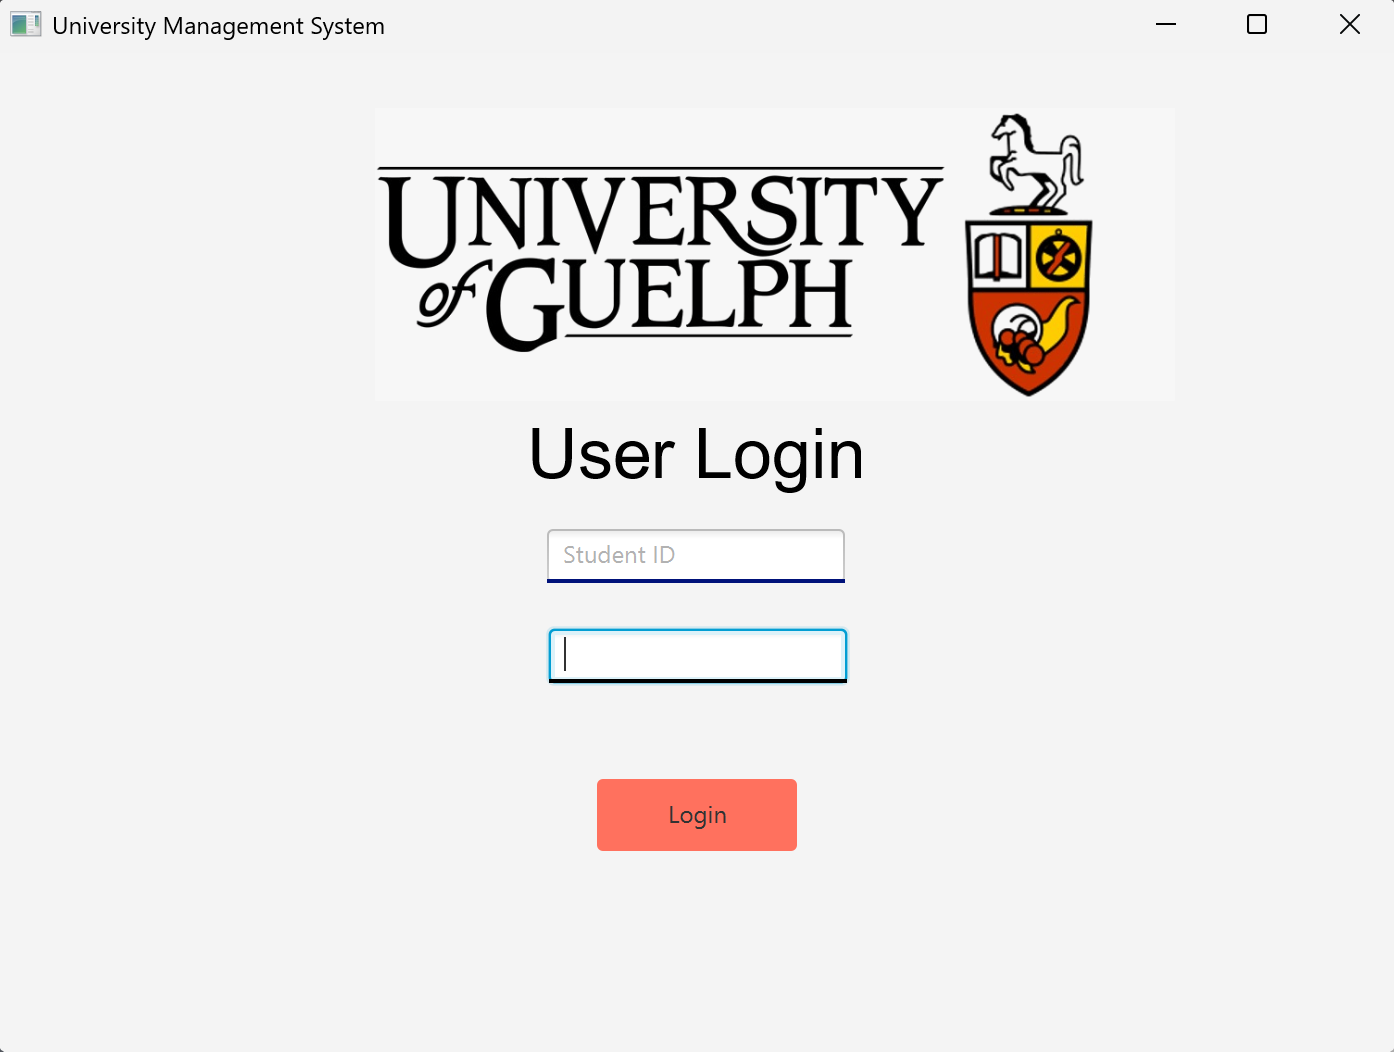
\includegraphics[width=1\linewidth]{figures/login_screen.png}
        \caption{Login Screen}
        \label{fig:example1}  
\end{figure}

% \subsection{Password Recovery (Optional)}


\subsection{First-Time Login Guide}

Once the user is at the login screen after running the program, they have either three login options to utilize the UMS program; faculty, student, and administrator. Each of these log-in credentials provides specific privileges that allow for editing such as deleting or adding, viewing, or changing personal settings. First time users must provide their correct login information in order to access the system, if they enter either an incorrect password or incorrect username, the user will receive an error message (see \autoref{fig:example2} below). This error will continue to occur until the user places the correct information, the user must login with the correct username and password; otherwise, it will continue to provide an error.


\begin{figure}[ht]
    \centering
        \centering
\includegraphics[width=1\linewidth]{figures/Incorrect_PW.png}
        \caption{Invalid Username/Password}
        \label{fig:example2}  
\end{figure}
\newpage
\section{Dashboard Overview}


\subsection{Admin Dashboard}


\subsubsection{Navigation Menu}


% \subsubsection{Quick Actions (Optional)}

\subsection{User Dashboard (Student/Faculty)}

\newpage
\section{Admin-Specific Features}

University Management system contains three main users that have access to this software, administrators, students, and faculty. Administrators are the users who have the highest level of privileges between all users with access to this software. They allow for the addition and deletion of specific features and users in the university management system.


\subsection{Subject Management}

The subject management tab allows administrators to add a specific subject to the University of Guelph. These subjects range between all the different departments for all the different colleges. Only administrators can make these changes as they have the required access and privileges to do so. In \autoref{fig:example5}, it showcases the subject management tab, in this tab administrators can either add a subject or delete a subject. First, adding a subject by entering their Subject Code and Subject Name, and deleting a subject by selecting the specific subject and clicking the red delete button. The removal of subjects comes from changes in the University Administration, low enrolment of students in a course, or changes in the overall program. \\

The process of adding and deleting a subject goes as follows.
\begin{enumerate}
    \item Administrator enters the Subject Code and the Subject Name
    \item Administrator press the Add Subject button
    \item Administrator review the table to ensure that the require course has been added
    \item Administrator can delete a course by selecting the targeted course resulting in a highlight. Then press the Delete Subject button.
    \item Data entries are saved in the integrated excel file.
\end{enumerate}

\textbf{Note:} The subject management tab is available for users such as faculty and students, however they do not have the ability to remove or add courses. They must have administrator login credentials for complete those tasks. 

\begin{figure}[h!]
    \centering
    \centering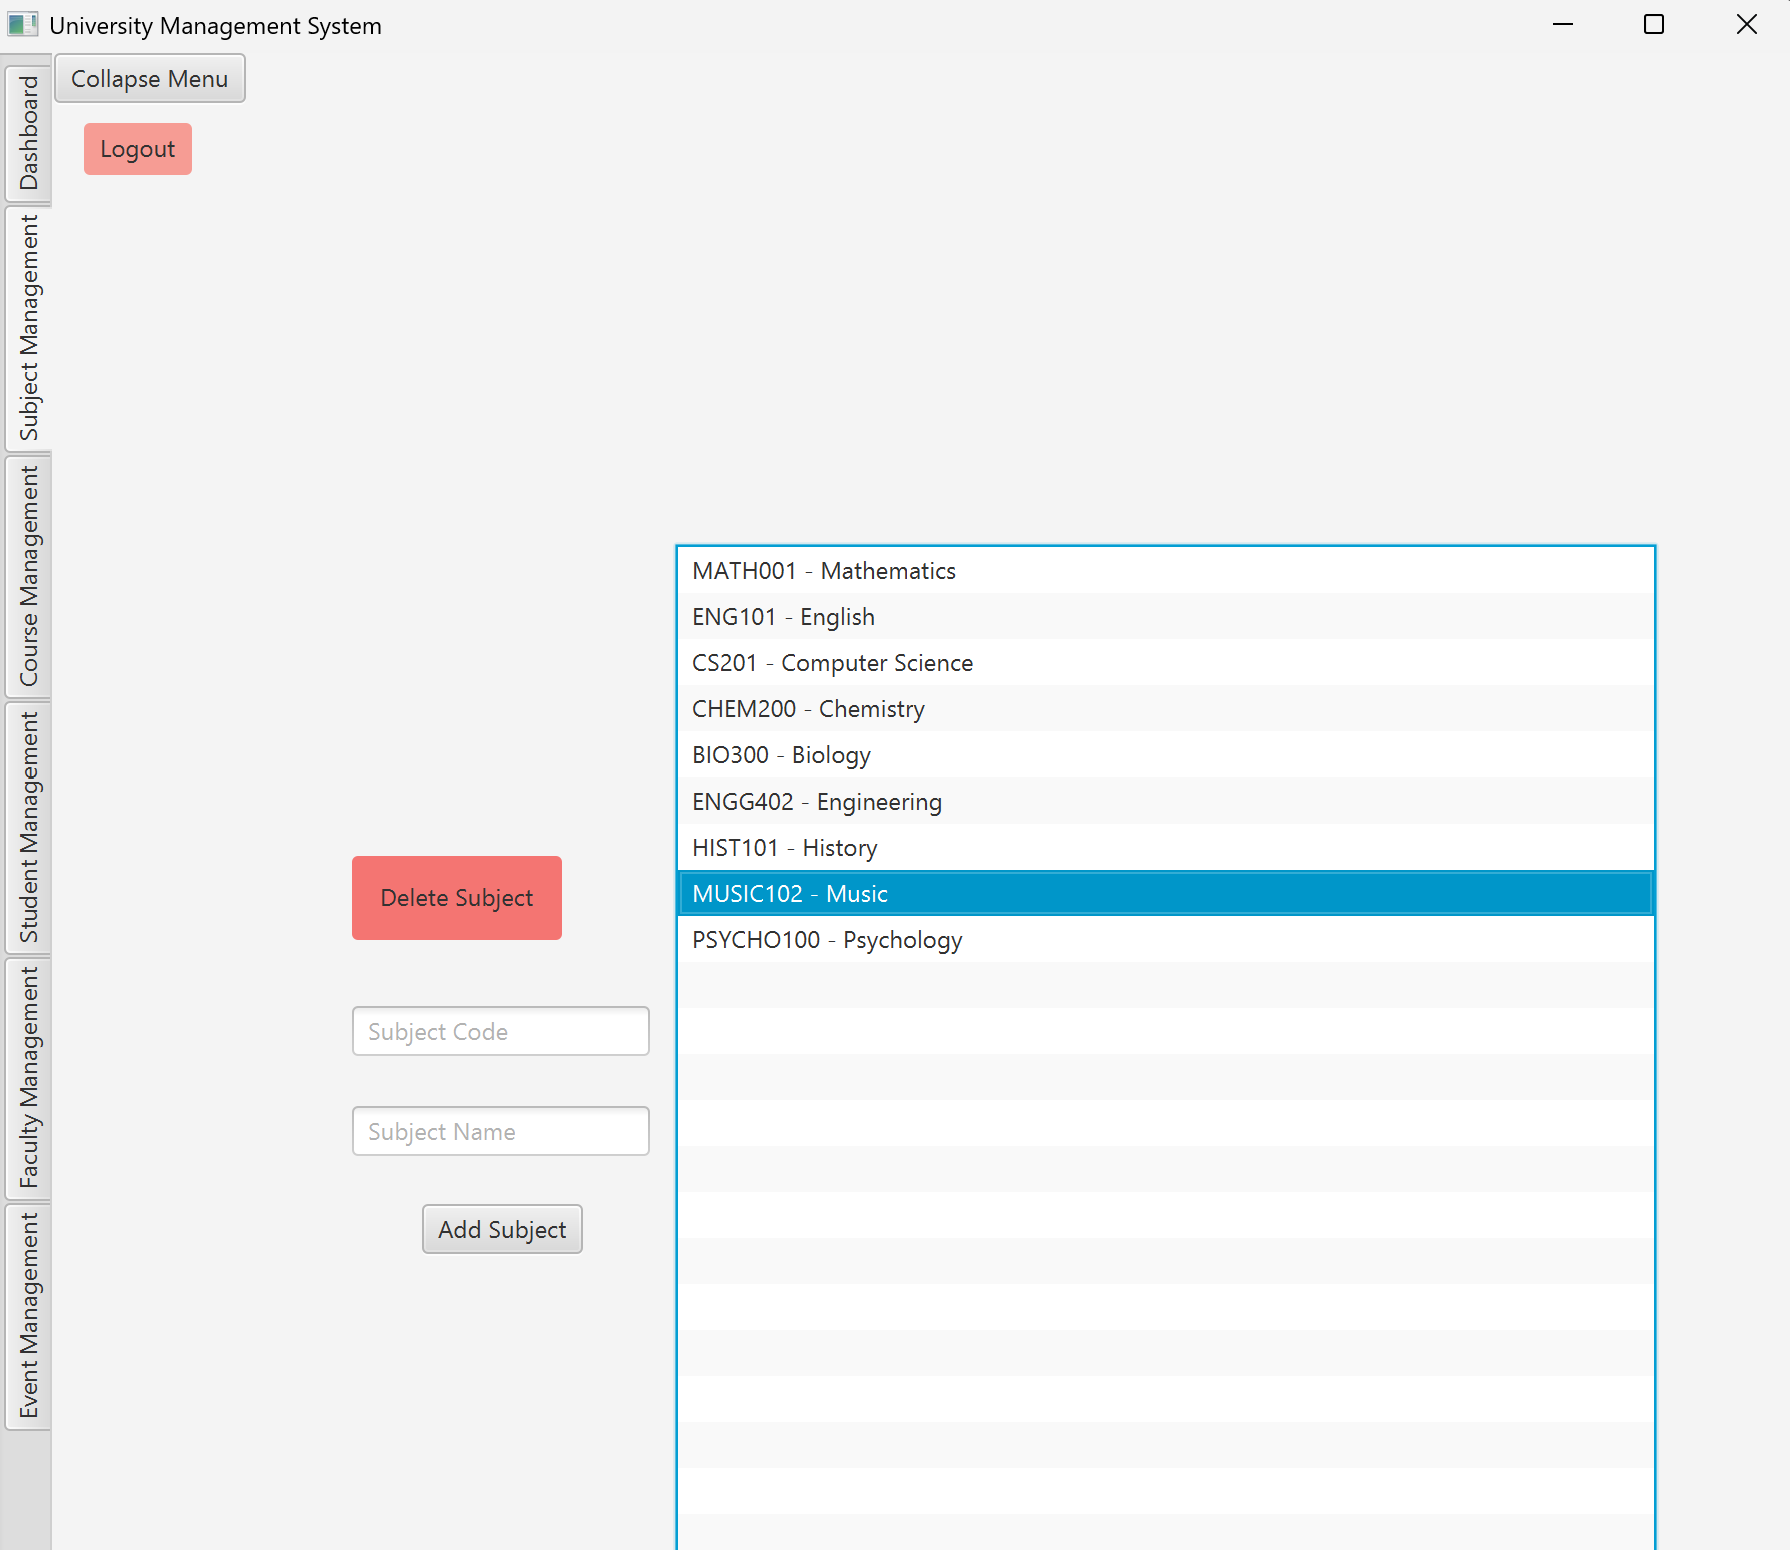
\includegraphics[width=0.7\linewidth]{figures/Subject_Management.png}
        \caption{Administrator Login - Subject Management Tab}
        \label{fig:example5} 
\end{figure}

\newpage
\subsection{Student Management}

The Student Management tab for administrators provides the administrator with the privilege of adding students to the University Management System, refer to \autoref{fig:example6} The procedure to add students is achieved by following the specific steps.

\begin{enumerate}
    \item Administrate clicks the input name field
    \item Administrator enters the student's name, email Student ID, and address, by clicking enter each time to store the information within the system and excel data archival file.
\end{enumerate}

\begin{figure}[h!]
    \centering
        \centering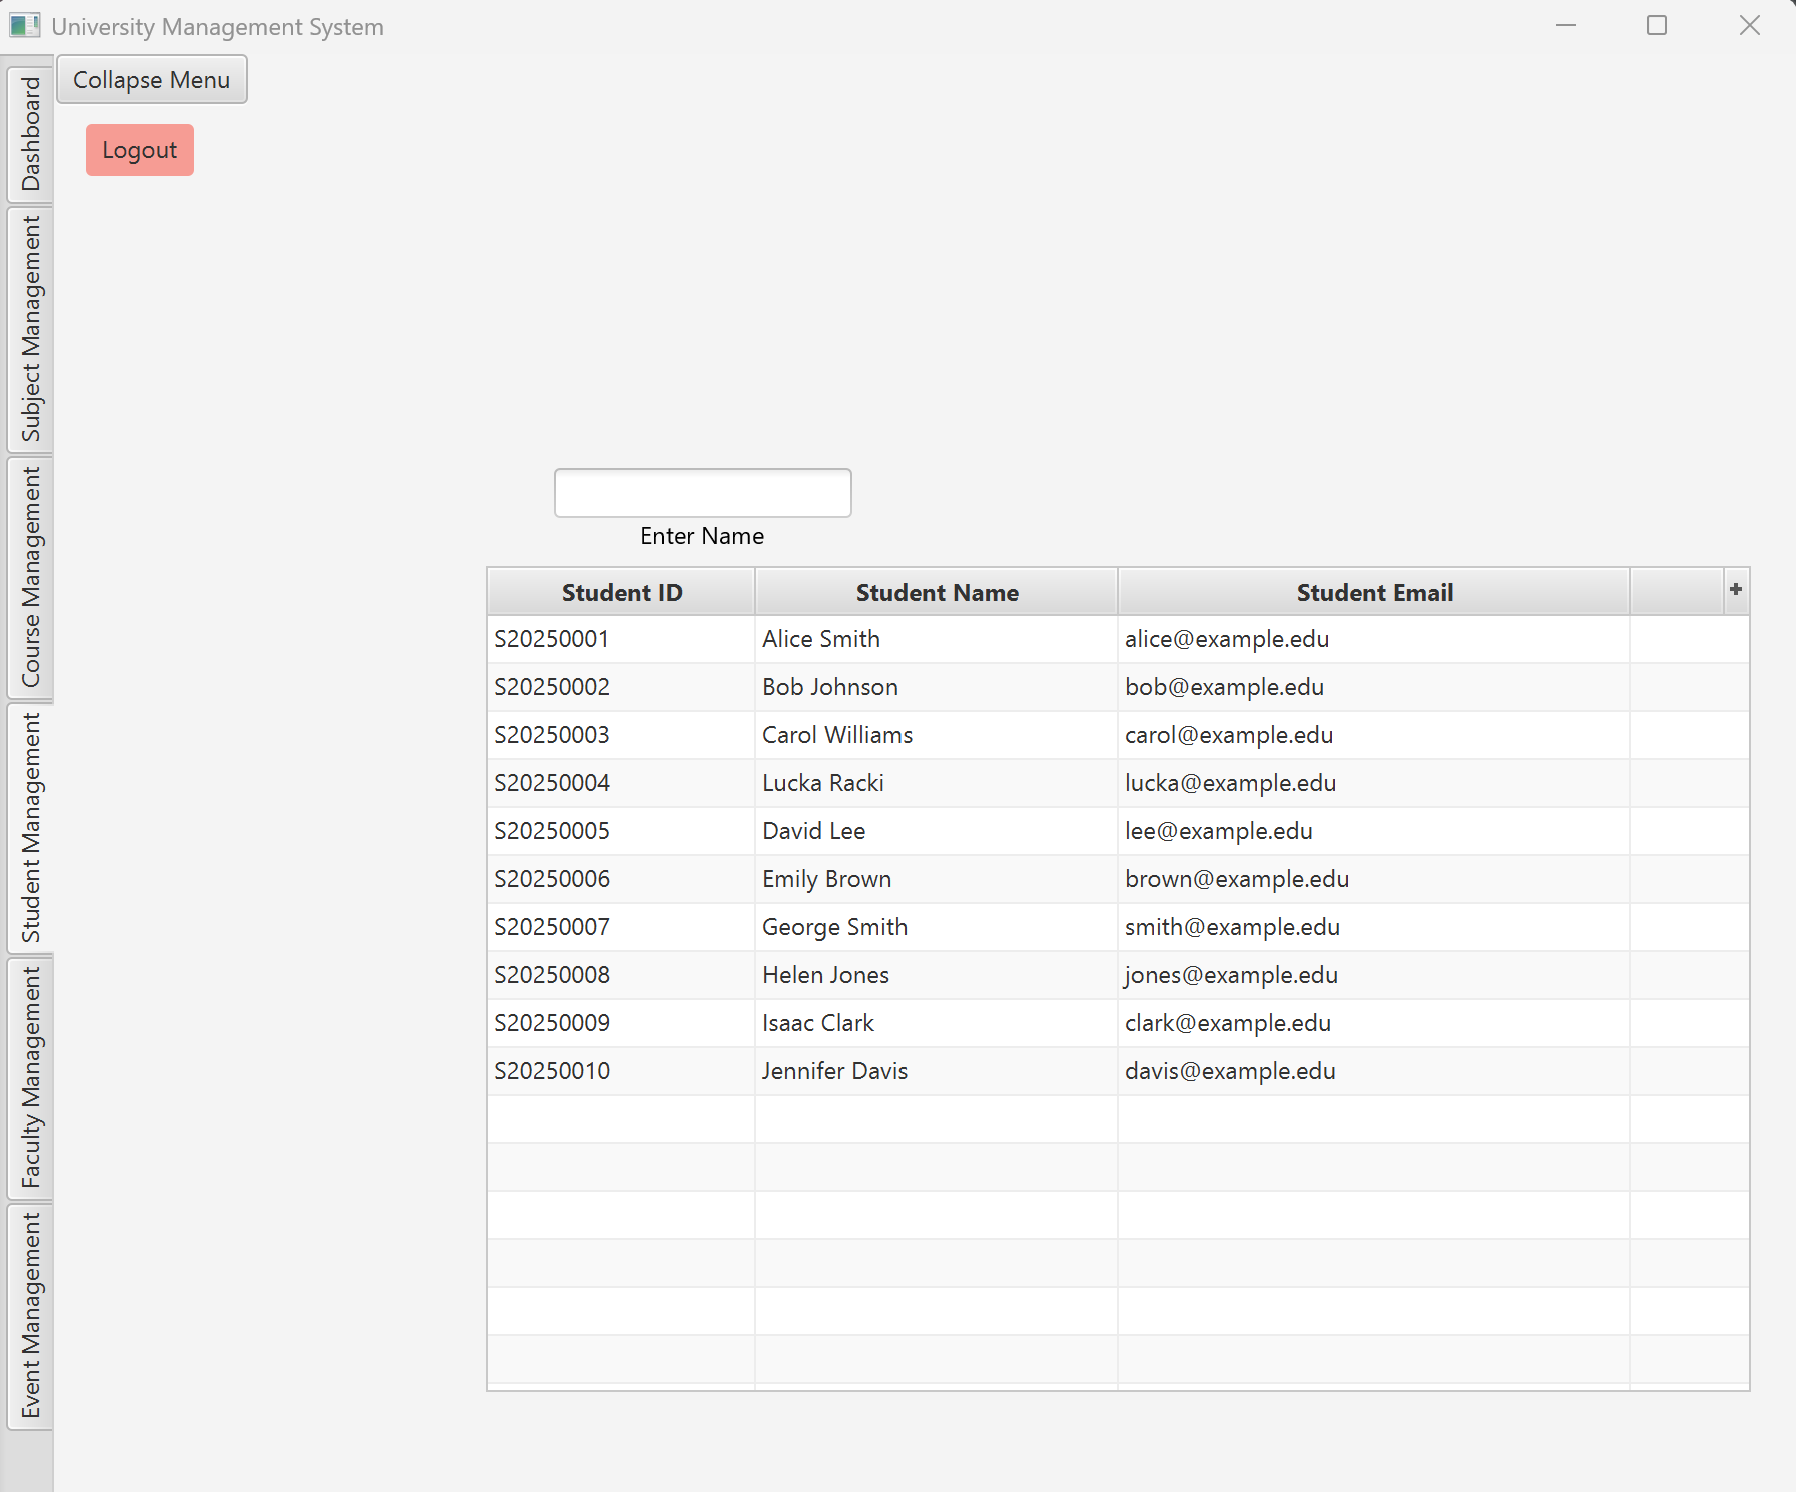
\includegraphics[width=0.7\linewidth]{figures/Student_Management.png}
        \caption{Administrator Login - Student Management Tab}
        \label{fig:example6}
        \FloatBarrier
\end{figure}


The Student Management tab also provides the capability to delete a student. However, this process requires that the administrator selects a student by double-clicking. This allows for a pop-up to occur proving the option to delete a student. Additionally, it provides their student information for the administrator privileges only. Refer to \autoref{fig:example7}.

\begin{figure}[ht!]
    \centering
        \centering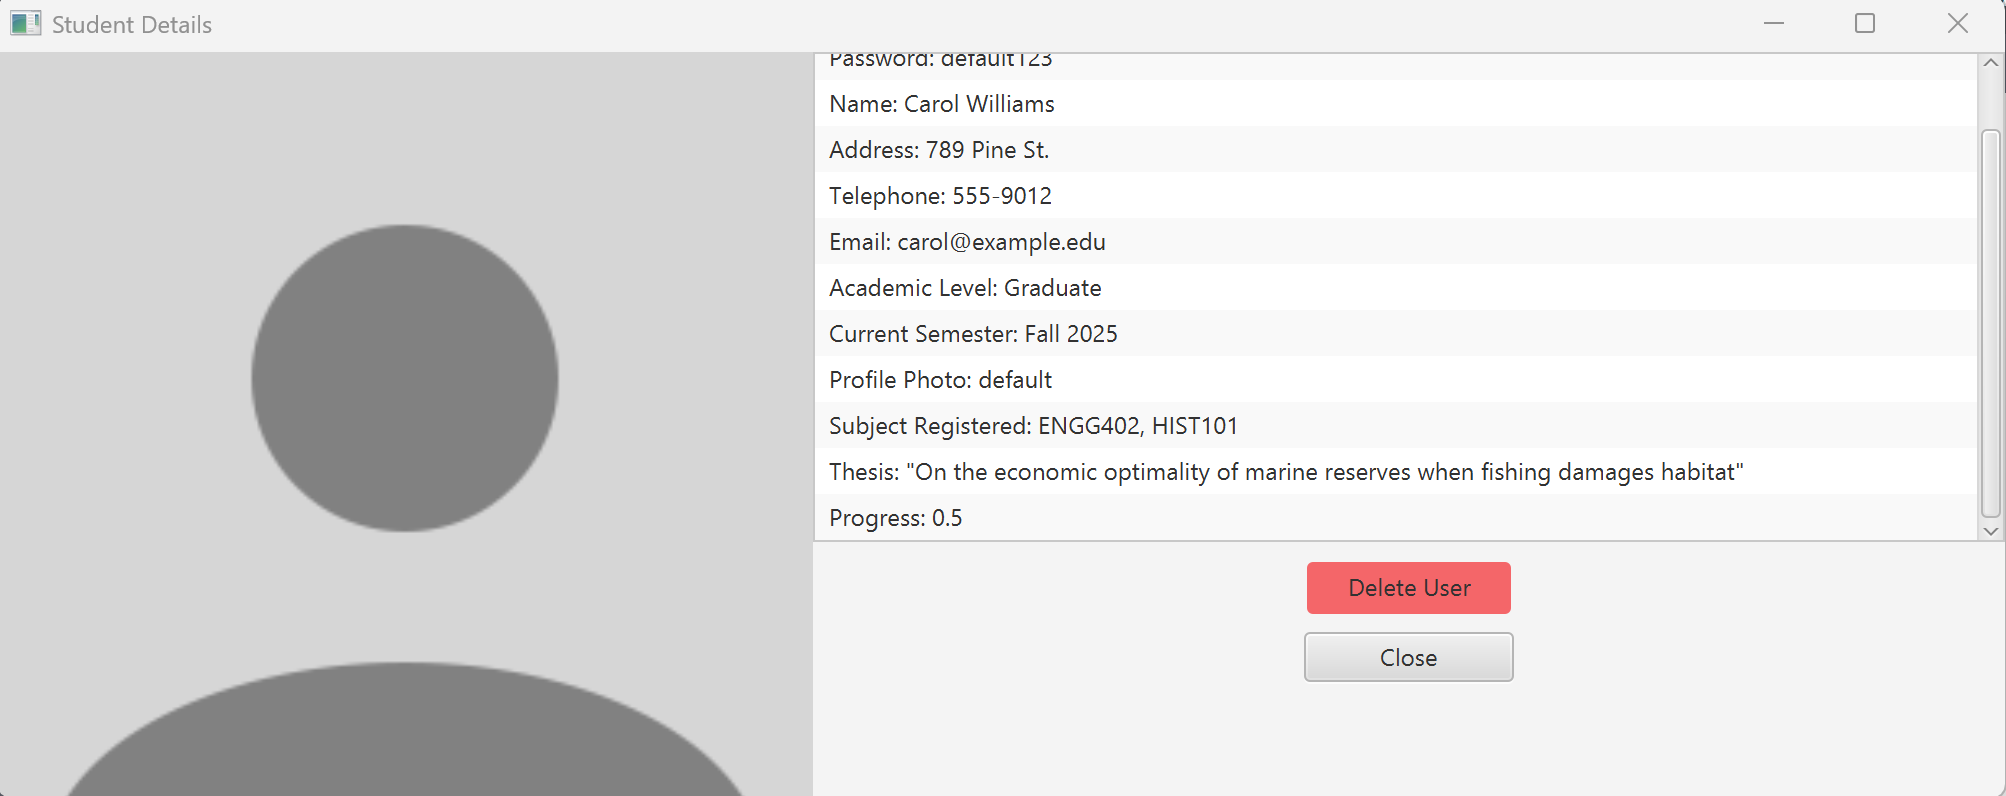
\includegraphics[width=1\linewidth]{figures/Student_Management_Delete.png}
        \caption{Administrator Login - Student Management Tab}
        \label{fig:example7}  
\end{figure}

\newpage
\subsection{Course Management}

The Course Management tab allows the administrator to add and delete courses for the University. Similar to the student management in order to add a course the administrator must utilize the input field box and enter the correct information. For example entering the correct, Course Name, Subject Code, Section Number, Capacity, Lecture Time. Final Exam Date, Location and Teacher. Once all these information have been added it will update in the table showcasing that it was a success.

Deleting a course requires the administrator to complete the following steps:
\begin{enumerate}
    \item Select designated course for deletion
    \item Press the delete course button
    \item Check if it is removed from thr excel data warehouse
\end{enumerate}

Note, that deleting a course is permanent and will require the user to input the same information again if it is deleted.

\begin{figure}[h]
    \centering
        \centering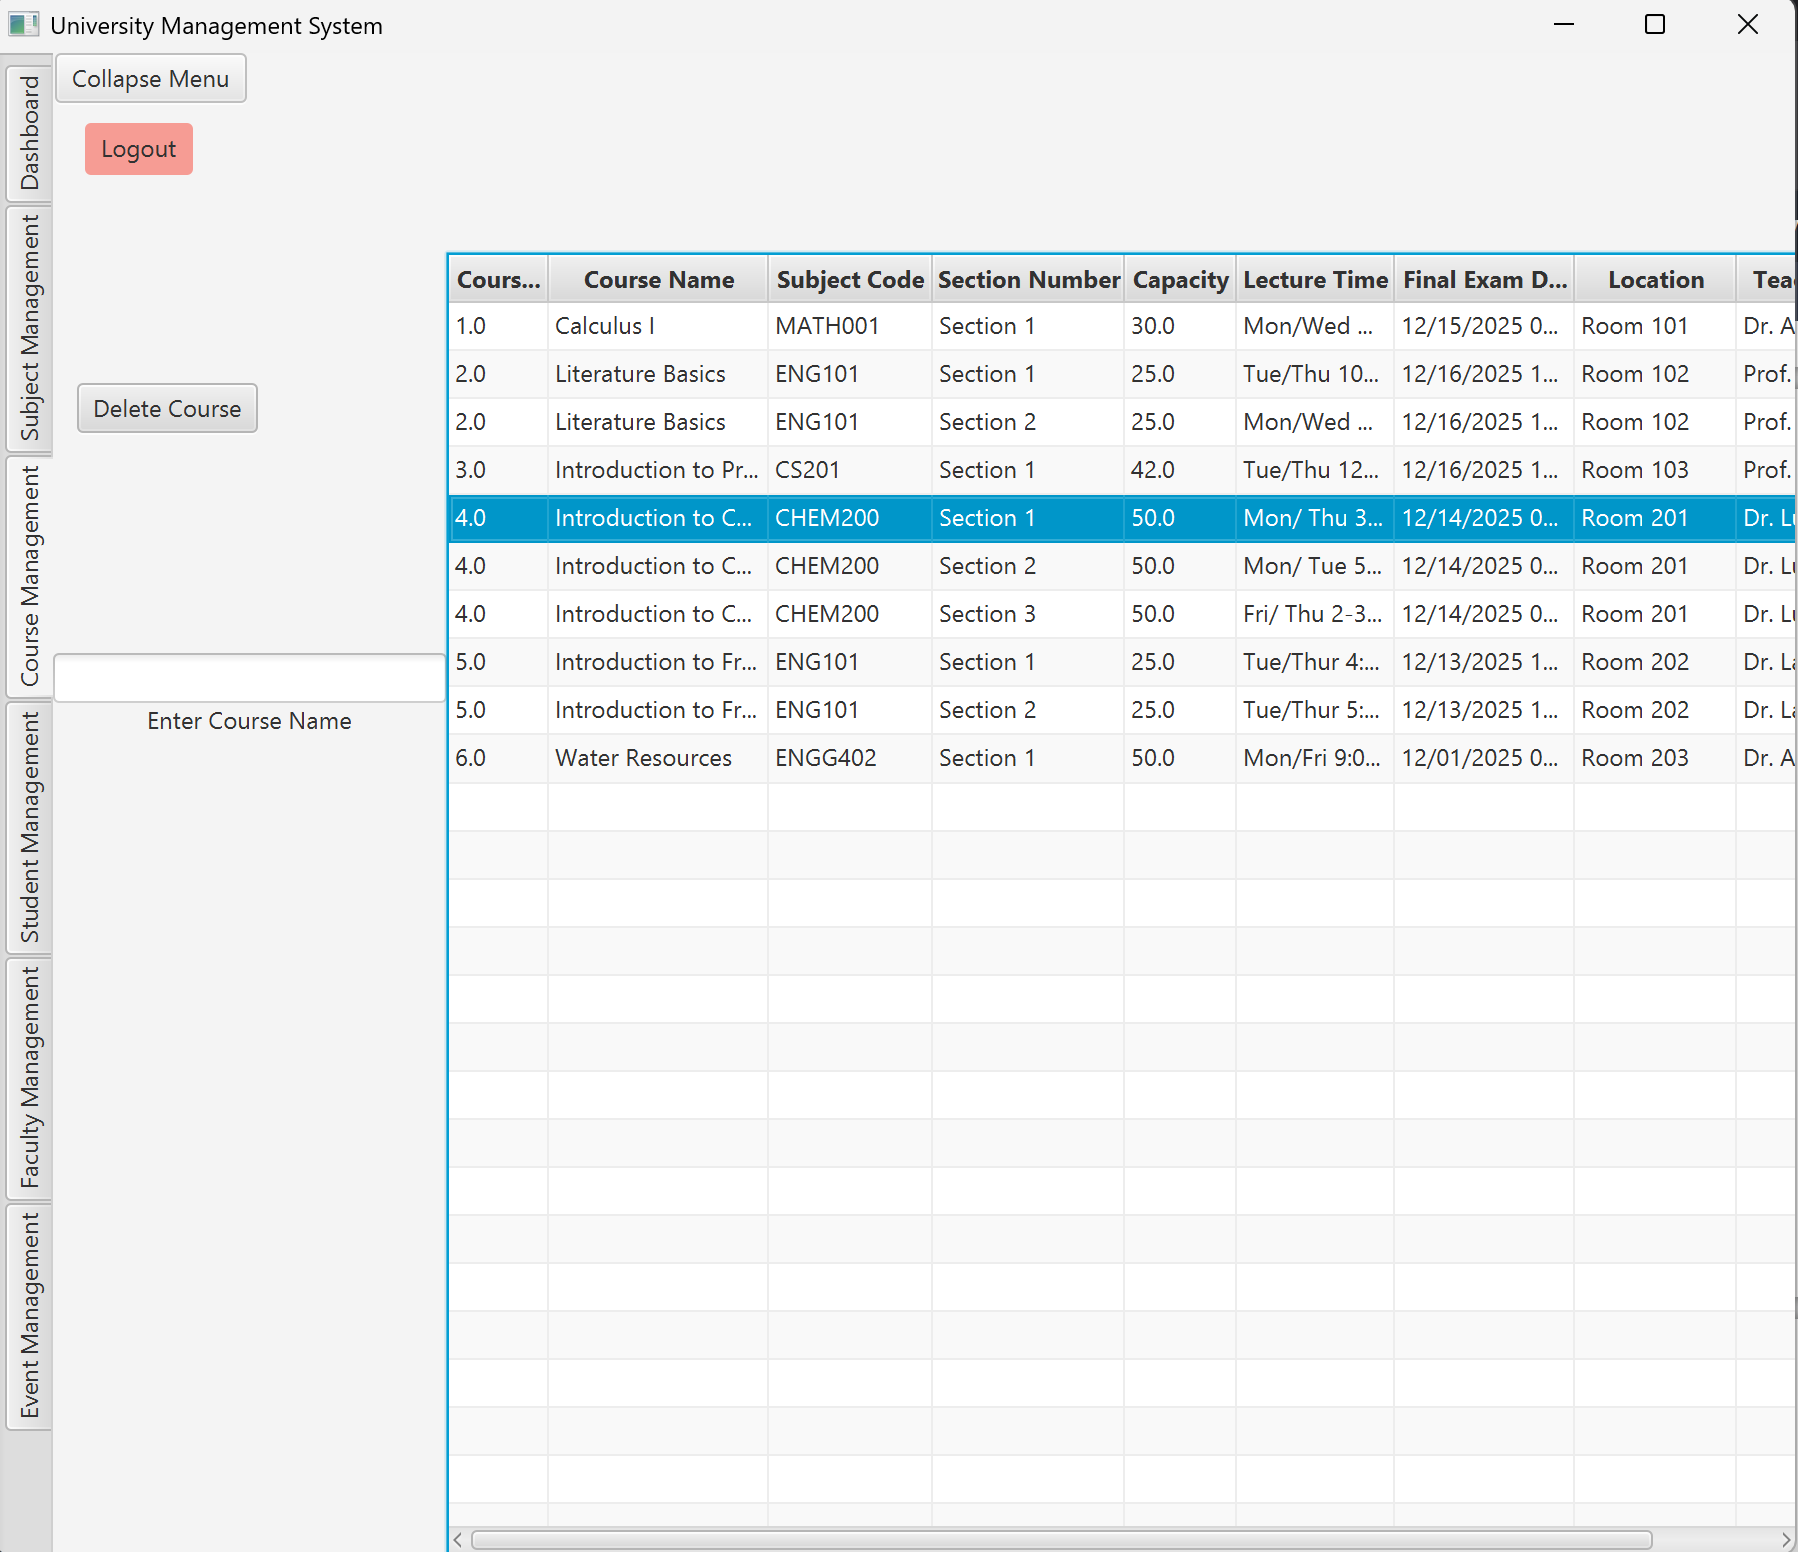
\includegraphics[width=1\linewidth]{figures/Course_Management.png}
        \caption{Administrator Login - Course Management Tab}
        % \label{fig:example11}  
\end{figure}


\subsection{Faculty Management}

The faculty management tab with the administrator login provides the capability to delete and add faculty members (see \autoref{fig:example9}). However, this requires that the course available exist from the course management tab, otherwise selecting the course offered is not possible. In order for an administrator to add a faculty member they must following these steps.

\begin{enumerate}
    \item Select the text box and add the name of the Faculty member
    \item Select the type of degree that they possess, assuming it is either Master's or Ph.D.
    \item Enter their Research interest
    \item Enter their Office Location
    \item Select the Course Offered drop down, assuming it is already included within the course management tab
    \item Press "Add Faculty" button, it will add the Faculty member in the data archive excel file
    \item Observe the added faculty member the in the provided table to the right.
\end{enumerate}


\begin{figure}[ht]
    \centering
        \centering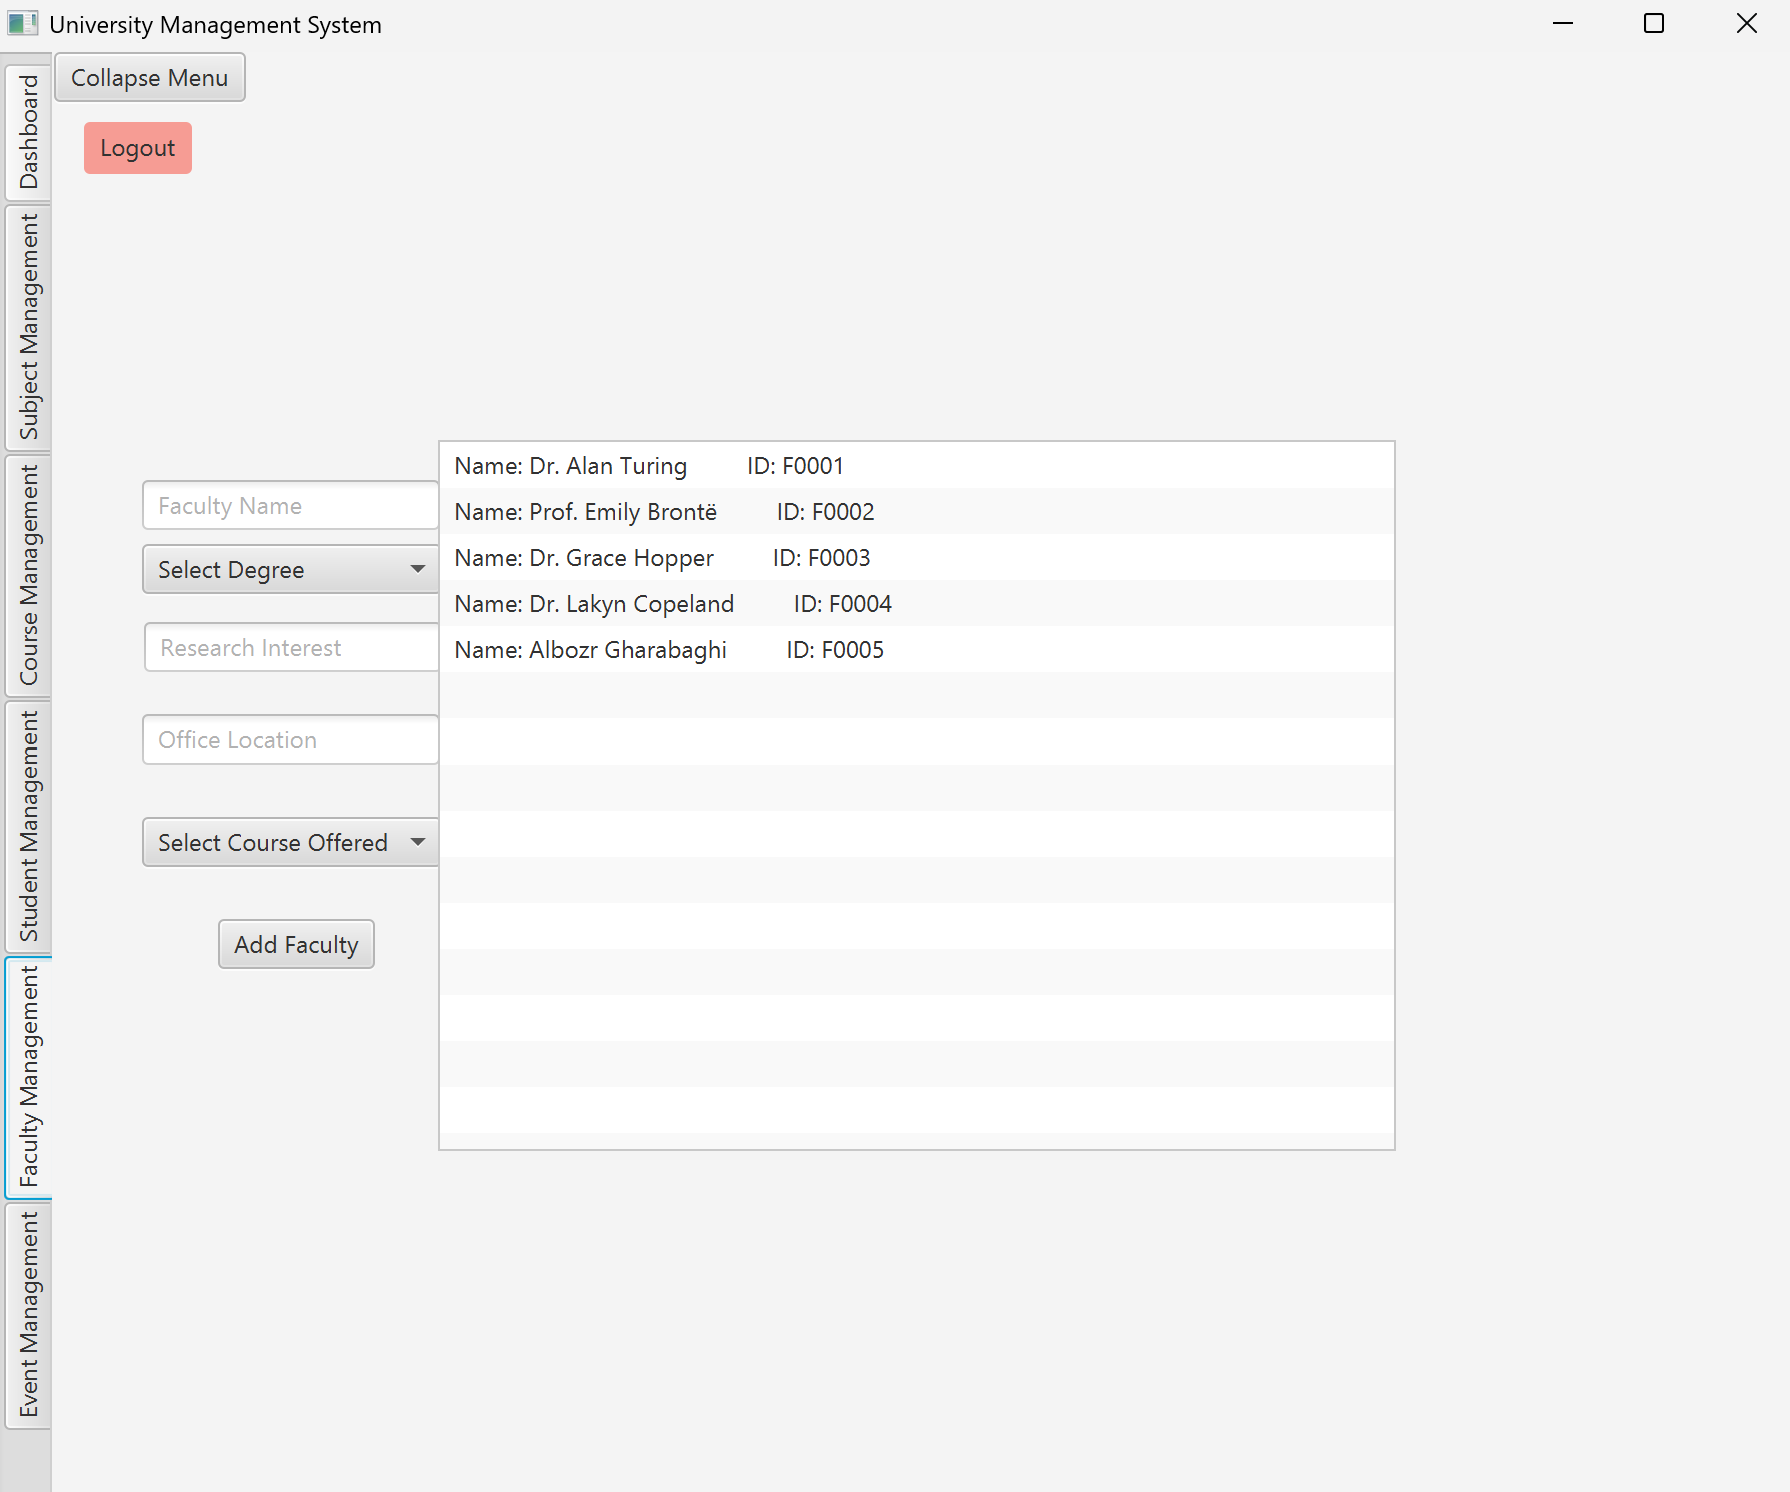
\includegraphics[width=1\linewidth]{figures/Faculty_Management.png}
        \caption{Administrator Login - Faculty Management Tab}
        \label{fig:example9}  
\end{figure}


\newpage
\subsection{Event Management}
The event management tab, focuses on adding events to the calendar that would be relevant to the overall University. This is placed allowing for both faculty and students to be notified on events. Administrators are the only users capable of adding events that remain relevant to the entire University (see \autoref{example10}). The process for adding an event is as follows:
\begin{enumerate}
    \item Enter the Event Date or click the calendar button to auto-select targeted date
    \item Enter the Event Name
    \item Enter the location
    \item Drag the total potential capacity, usually given within the budget or safety protocol
    \item Drag the cost, notice that the it snaps to the closest value of plus minus 0.25, 0.5, 0.75, 1.0
    \item Drag the time it would take for the event, notice it snaps to the closest value rounded by a quarter
    \item Add the event, this should be place in the calendar depending on the selected date.
    
\end{enumerate}

\begin{figure}[ht]
    \centering
        \centering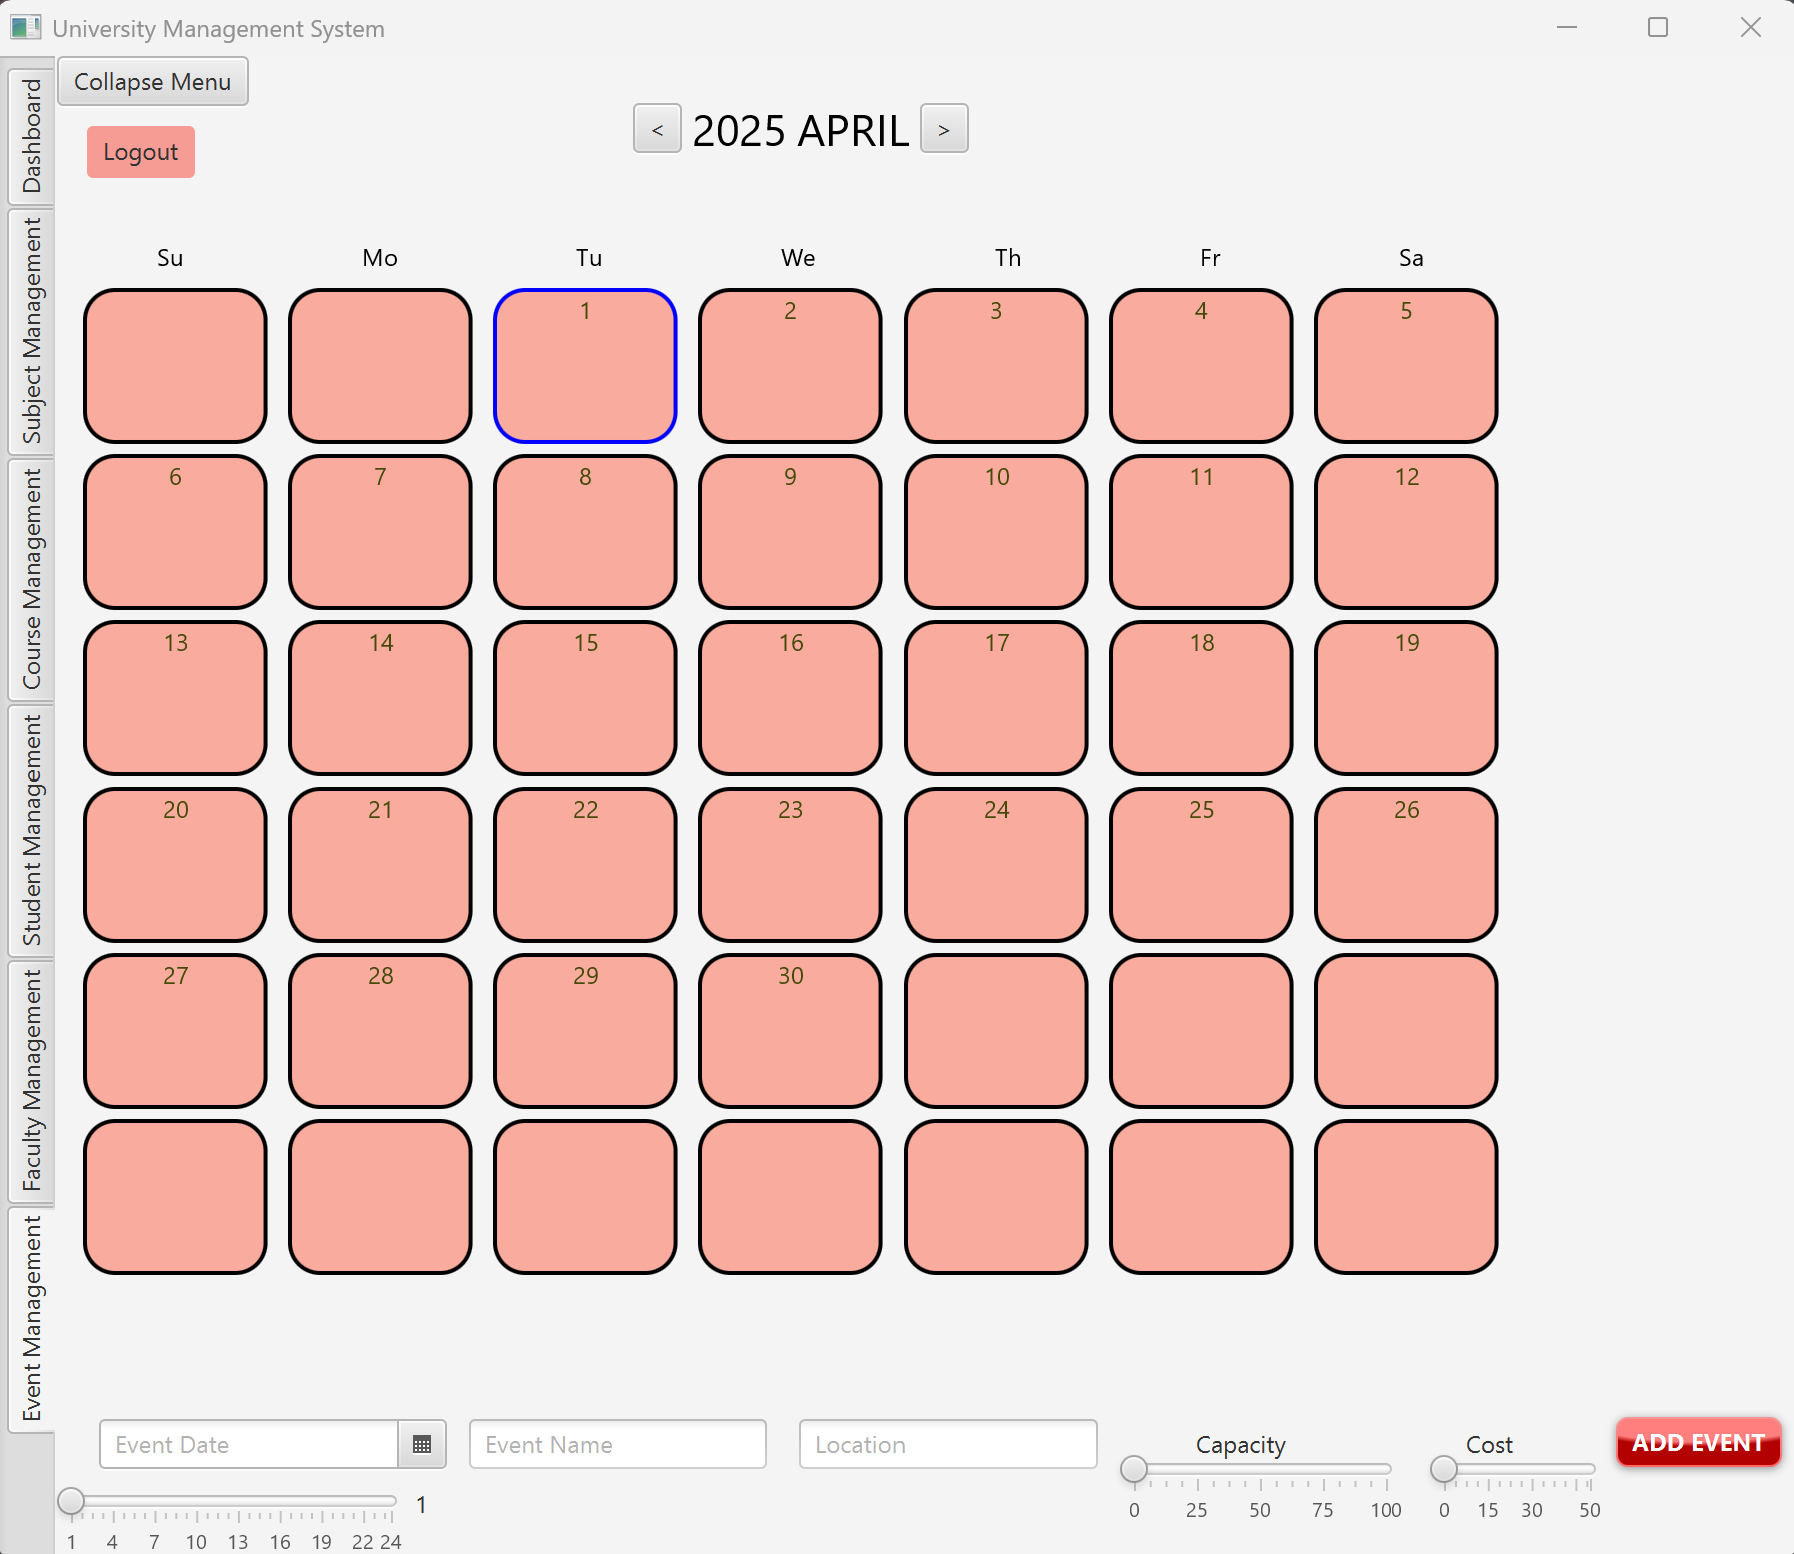
\includegraphics[width=1\linewidth]{figures/Event_Management.png}
        \caption{Administrator Login - Event Management Tab}
        \label{fig:example10}  
\end{figure}
\newpage
\section{User-Specific Features (Students/Faculty)}

User-Specific features are dependent on whether the user logs in as a student or a faculty. Faculty members will have different privileges and information than student.


% \subsection{Subject Management Tab}

% \lipsum[9]

% \begin{figure}[ht]
%     \centering
%         \centering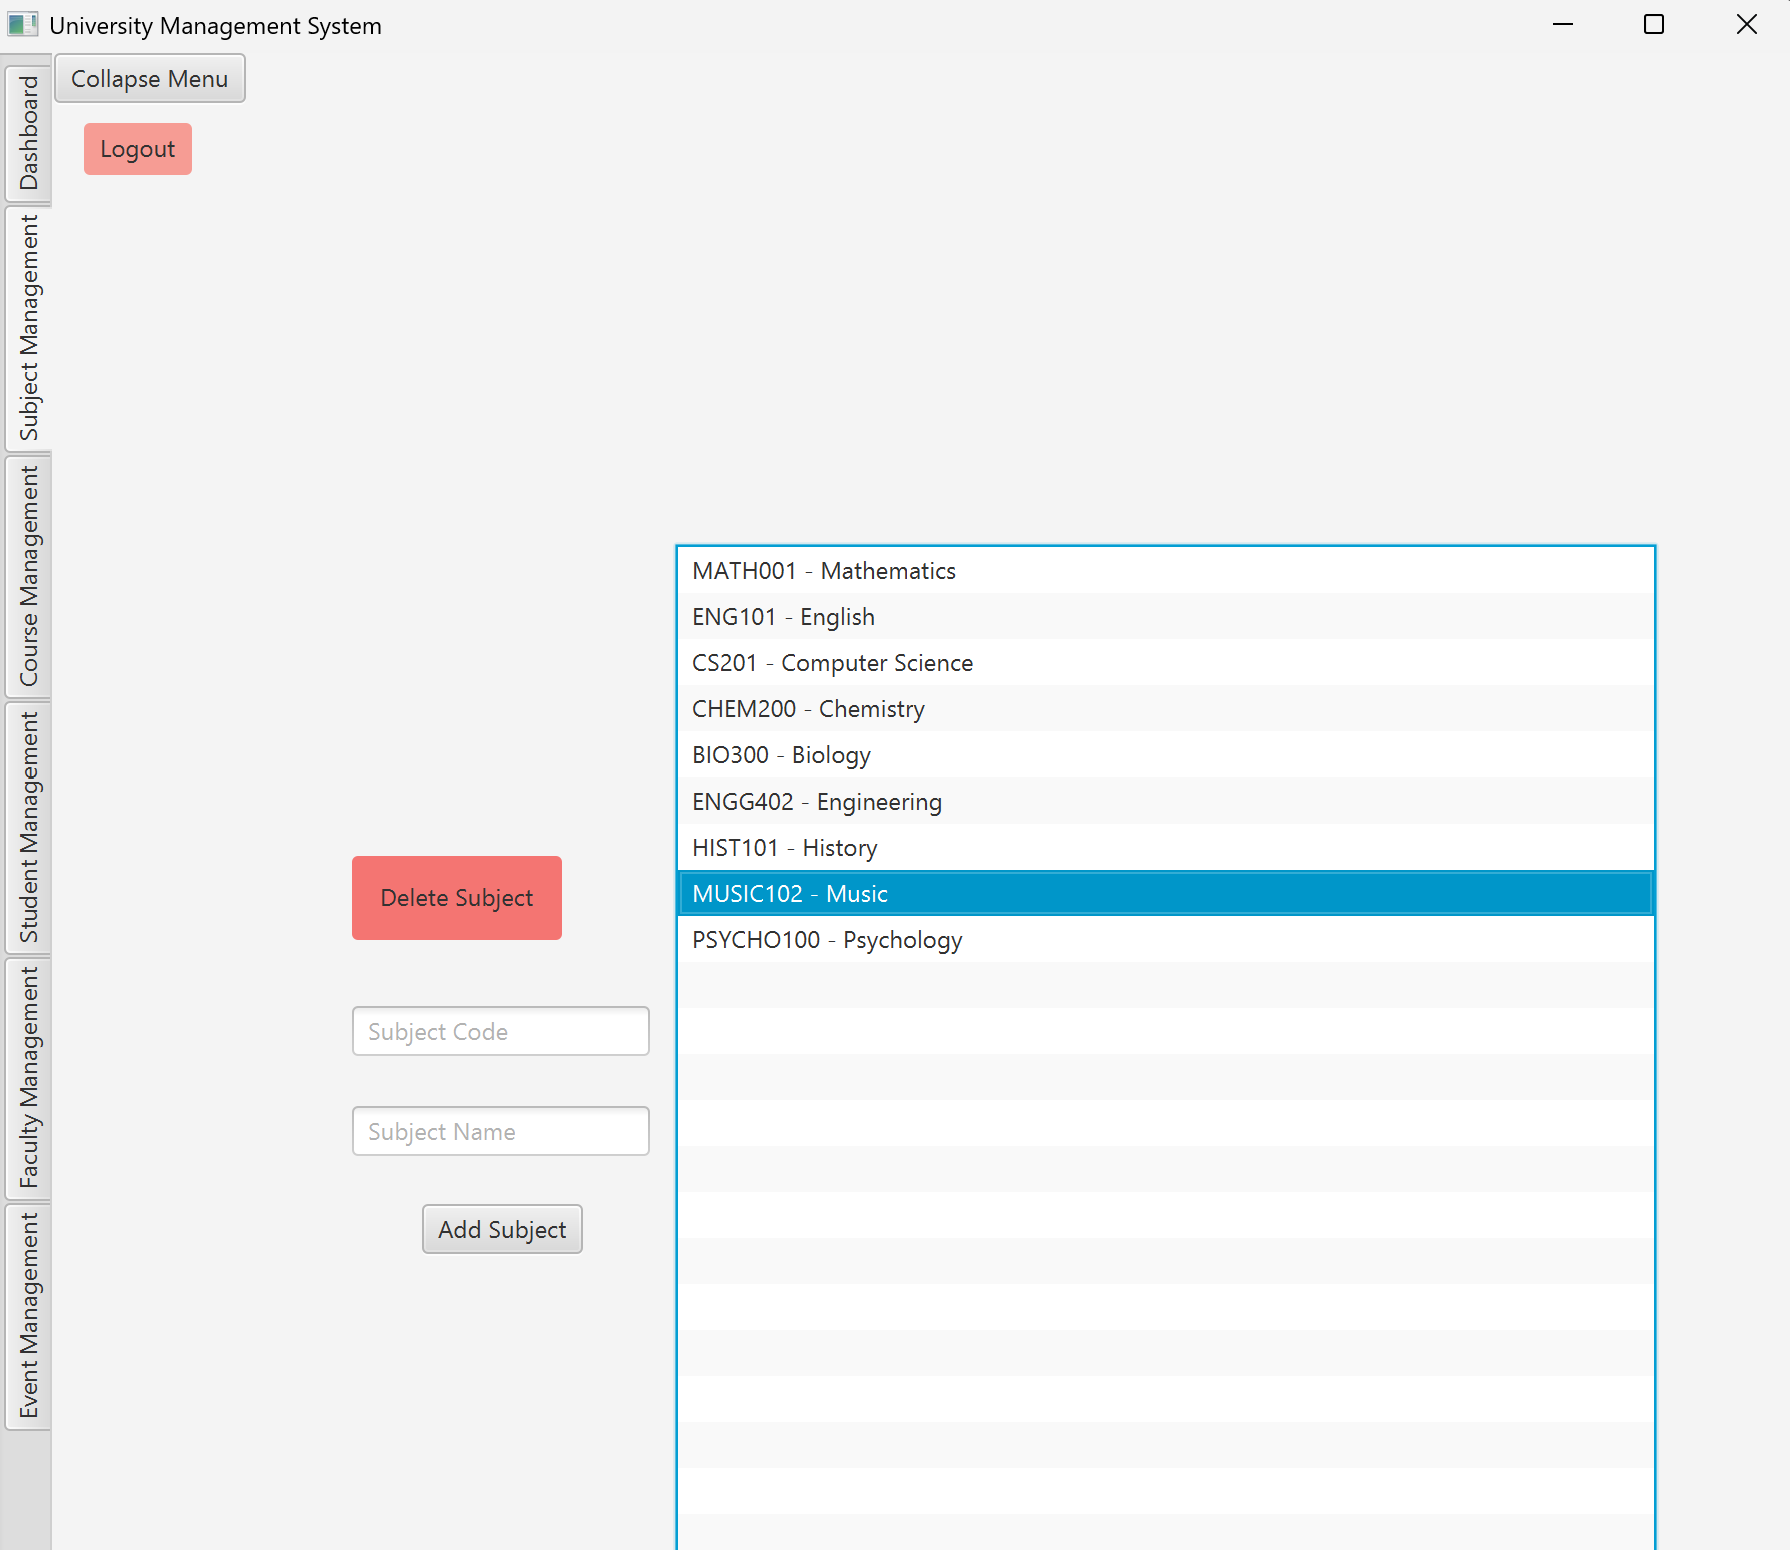
\includegraphics[width=1\linewidth]{figures/Subject_Management.png}
%         \caption{Subject Management}
%         % \label{fig:example11}  
% \end{figure}

\subsection{Course Management Tab}

\lipsum[9]

\newpage
\subsubsection{Student View}

\lipsum[9]

\begin{figure}[ht]
    \centering
        \centering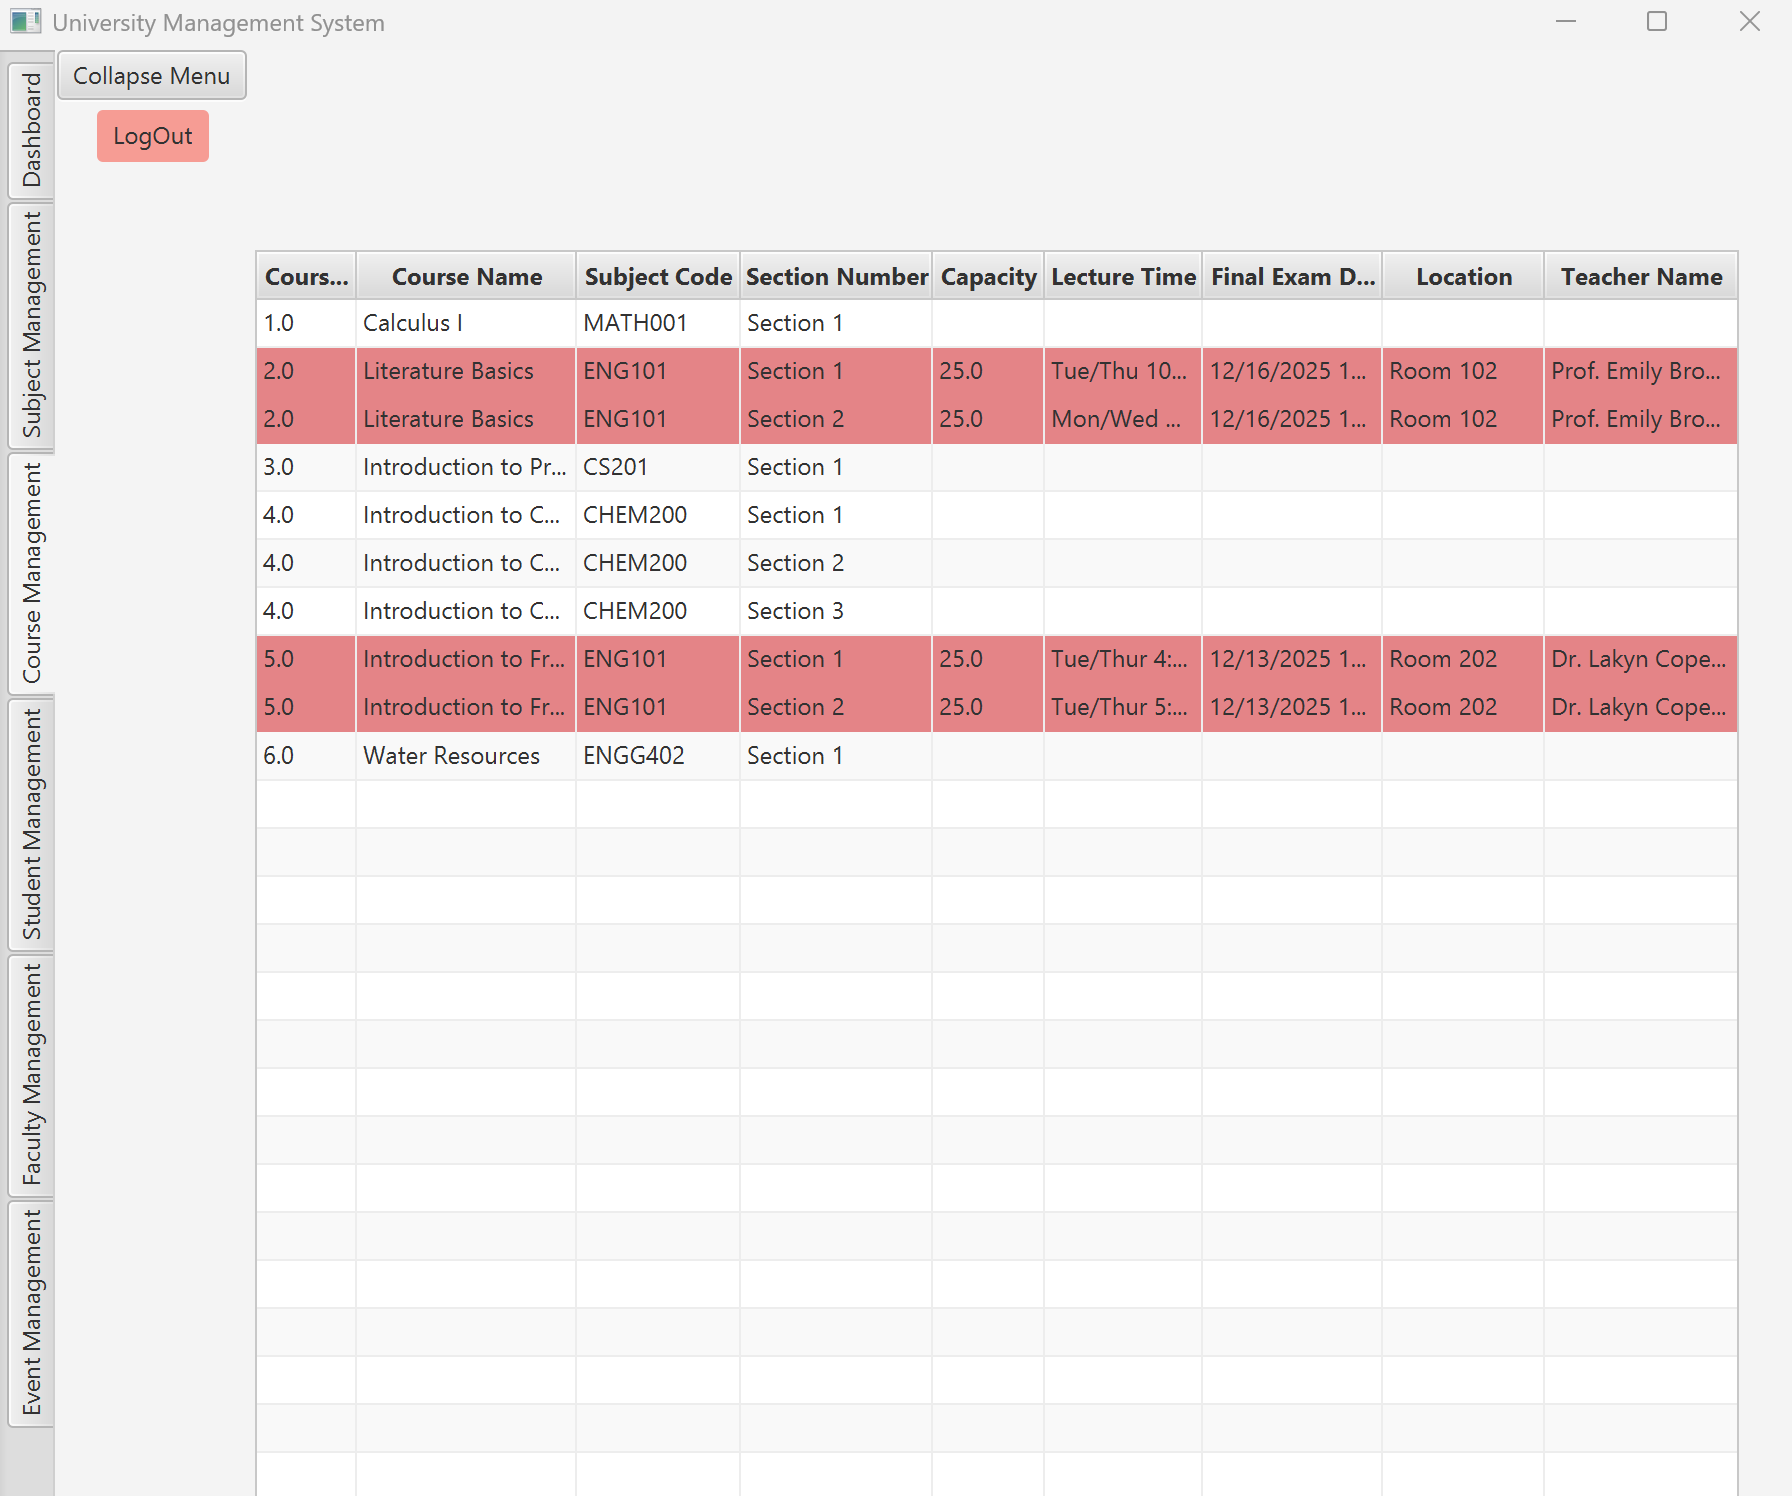
\includegraphics[width=0.7\linewidth]{figures/STD_Course_Management_Tab.png}
        \caption{Student Login - Course Management}
        % \label{fig:example11}  
        \FloatBarrier
\end{figure}


\subsubsection{Faculty View}
\lipsum[9]

\begin{figure}[ht]
    \centering
        \centering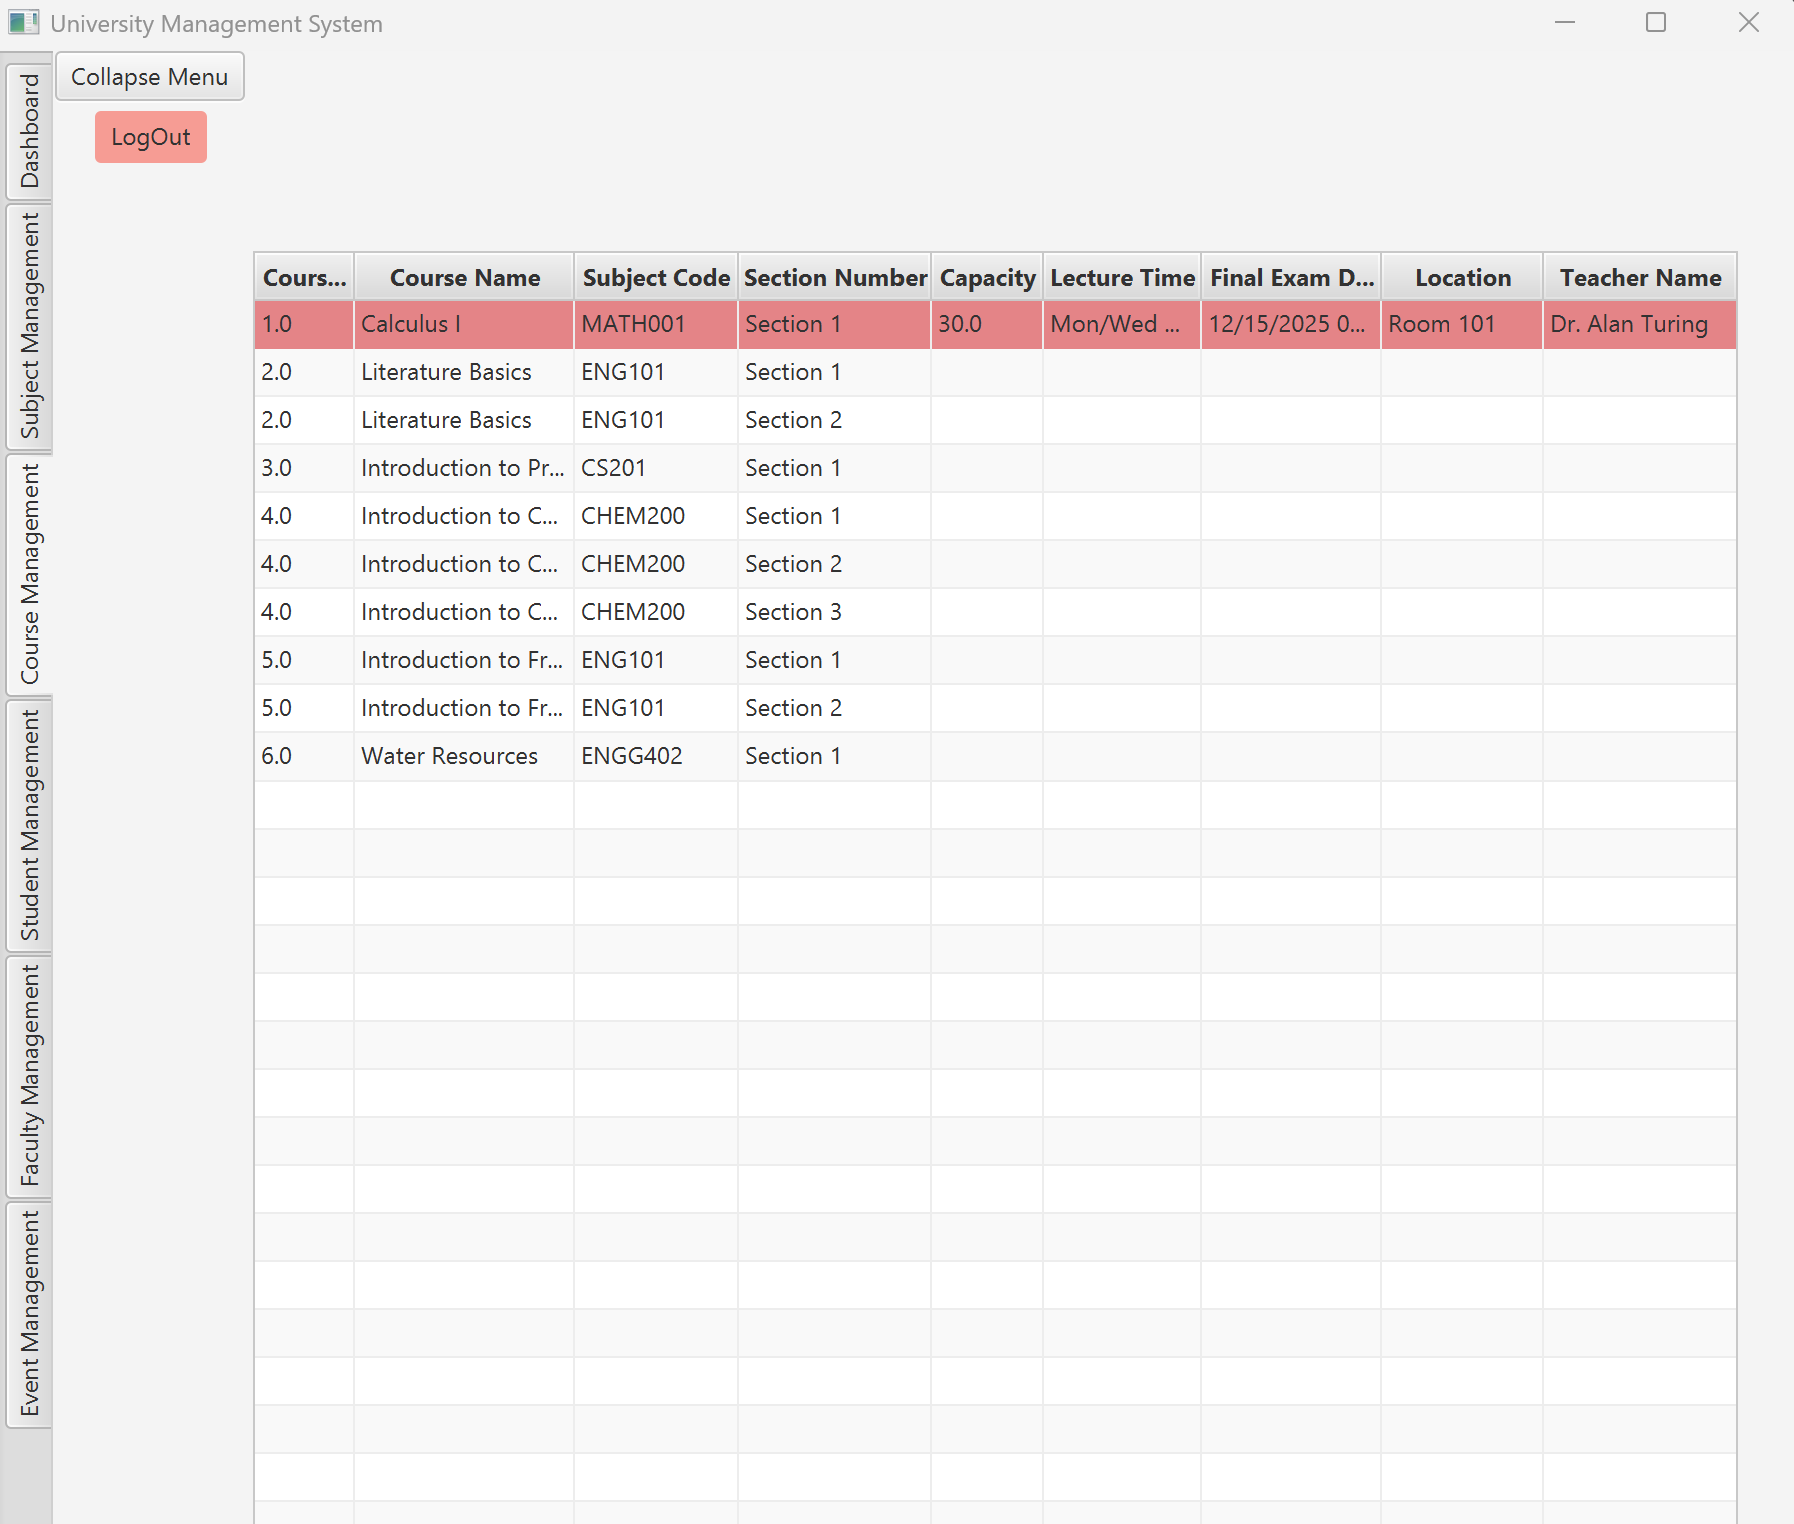
\includegraphics[width=0.7\linewidth]{figures/FAC_Course_Management_Tab.png}
        \caption{Faculty Login - Course Management}
        % \label{fig:example11}  
\end{figure}

\newpage
\subsection{Student Management Tab}

\lipsum[9]


\subsubsection{Student View}

\lipsum[9]

\begin{figure}[ht]
    \centering
        \centering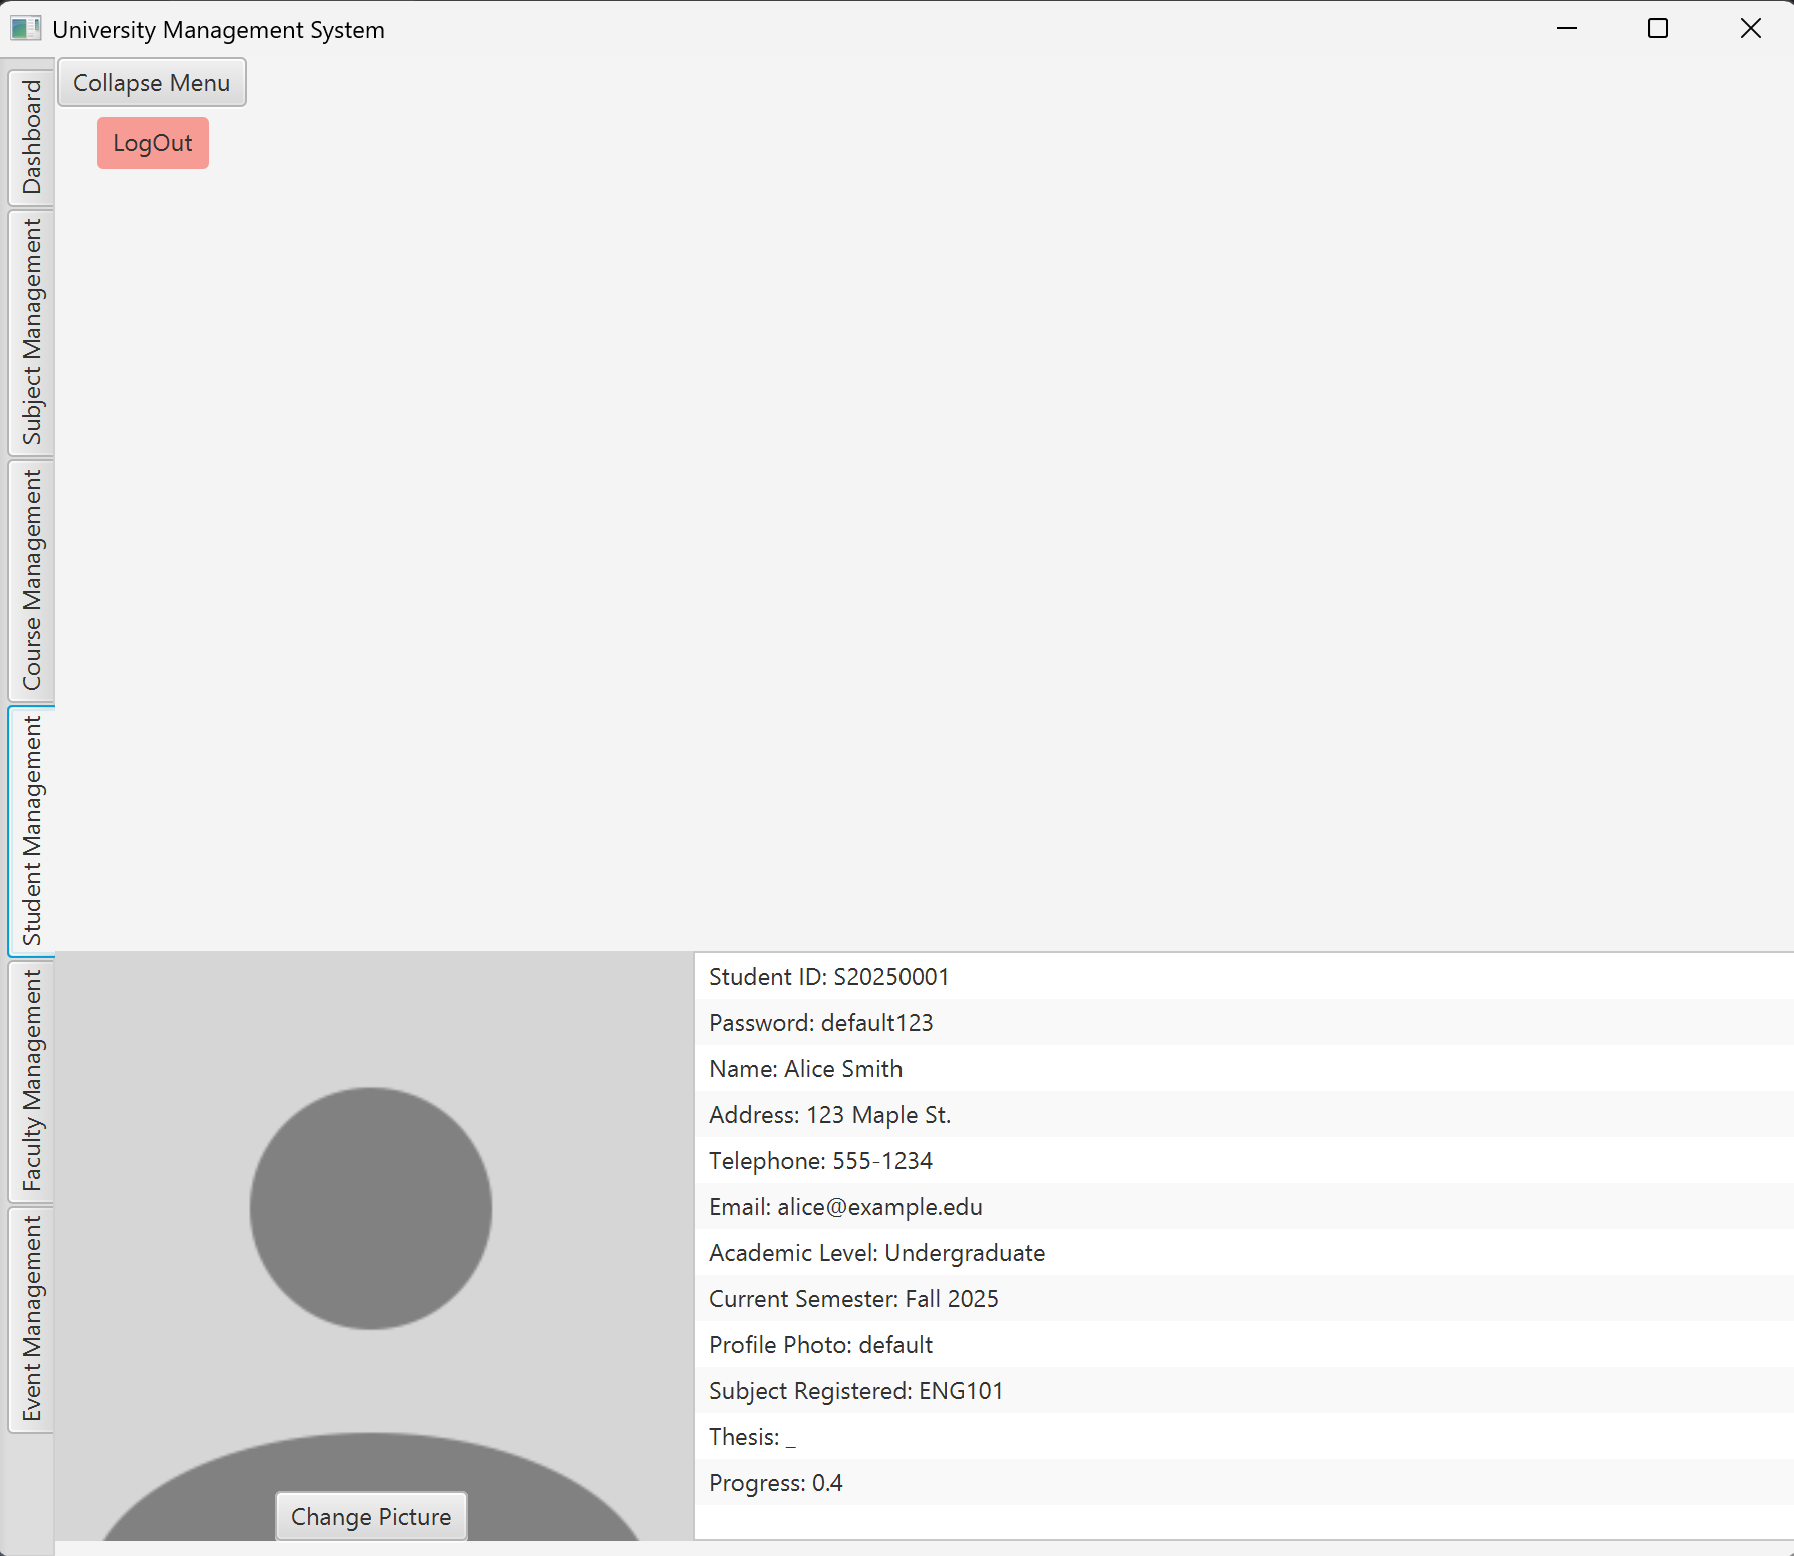
\includegraphics[width=0.65\linewidth]{figures/STD_Student_Management_Tab.png}
        \caption{Student Login - Student Management Tab}
        % \label{fig:example11}  
\end{figure}

\newpage
\subsubsection{Faculty View}

\lipsum[9]


\begin{figure}[ht]
    \centering
        \centering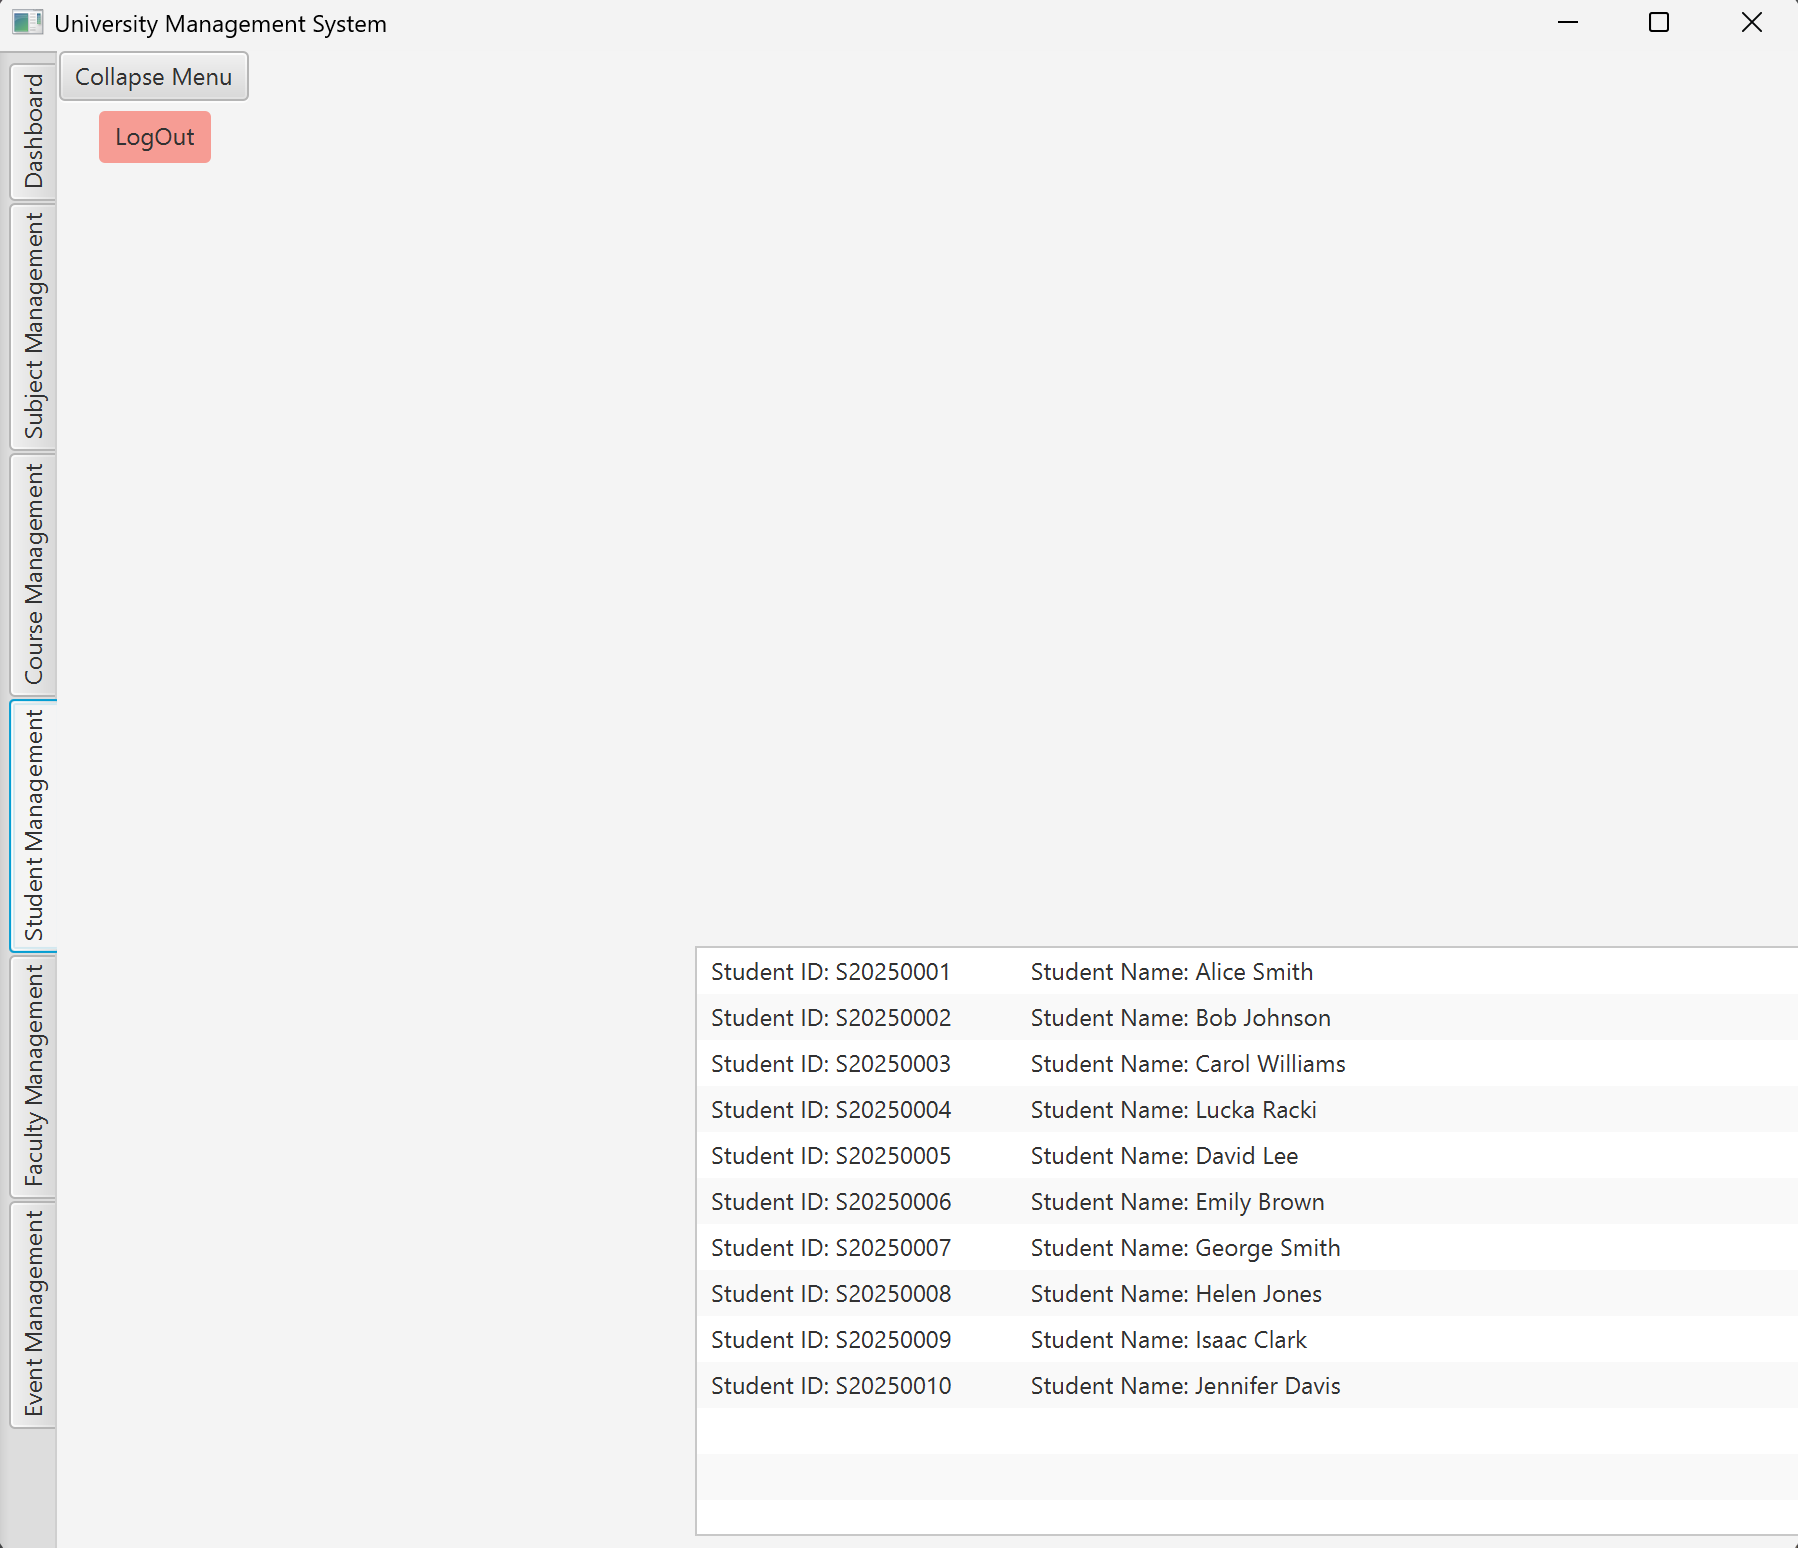
\includegraphics[width=0.7\linewidth]{figures/FAC_Student_Management_Tab.png}
        \caption{Faculty Login - Student Management Tab}
        % \label{fig:example11}  
\end{figure}

% \subsubsection{Student View}

% \begin{figure}[ht]
%     \centering
%         \centering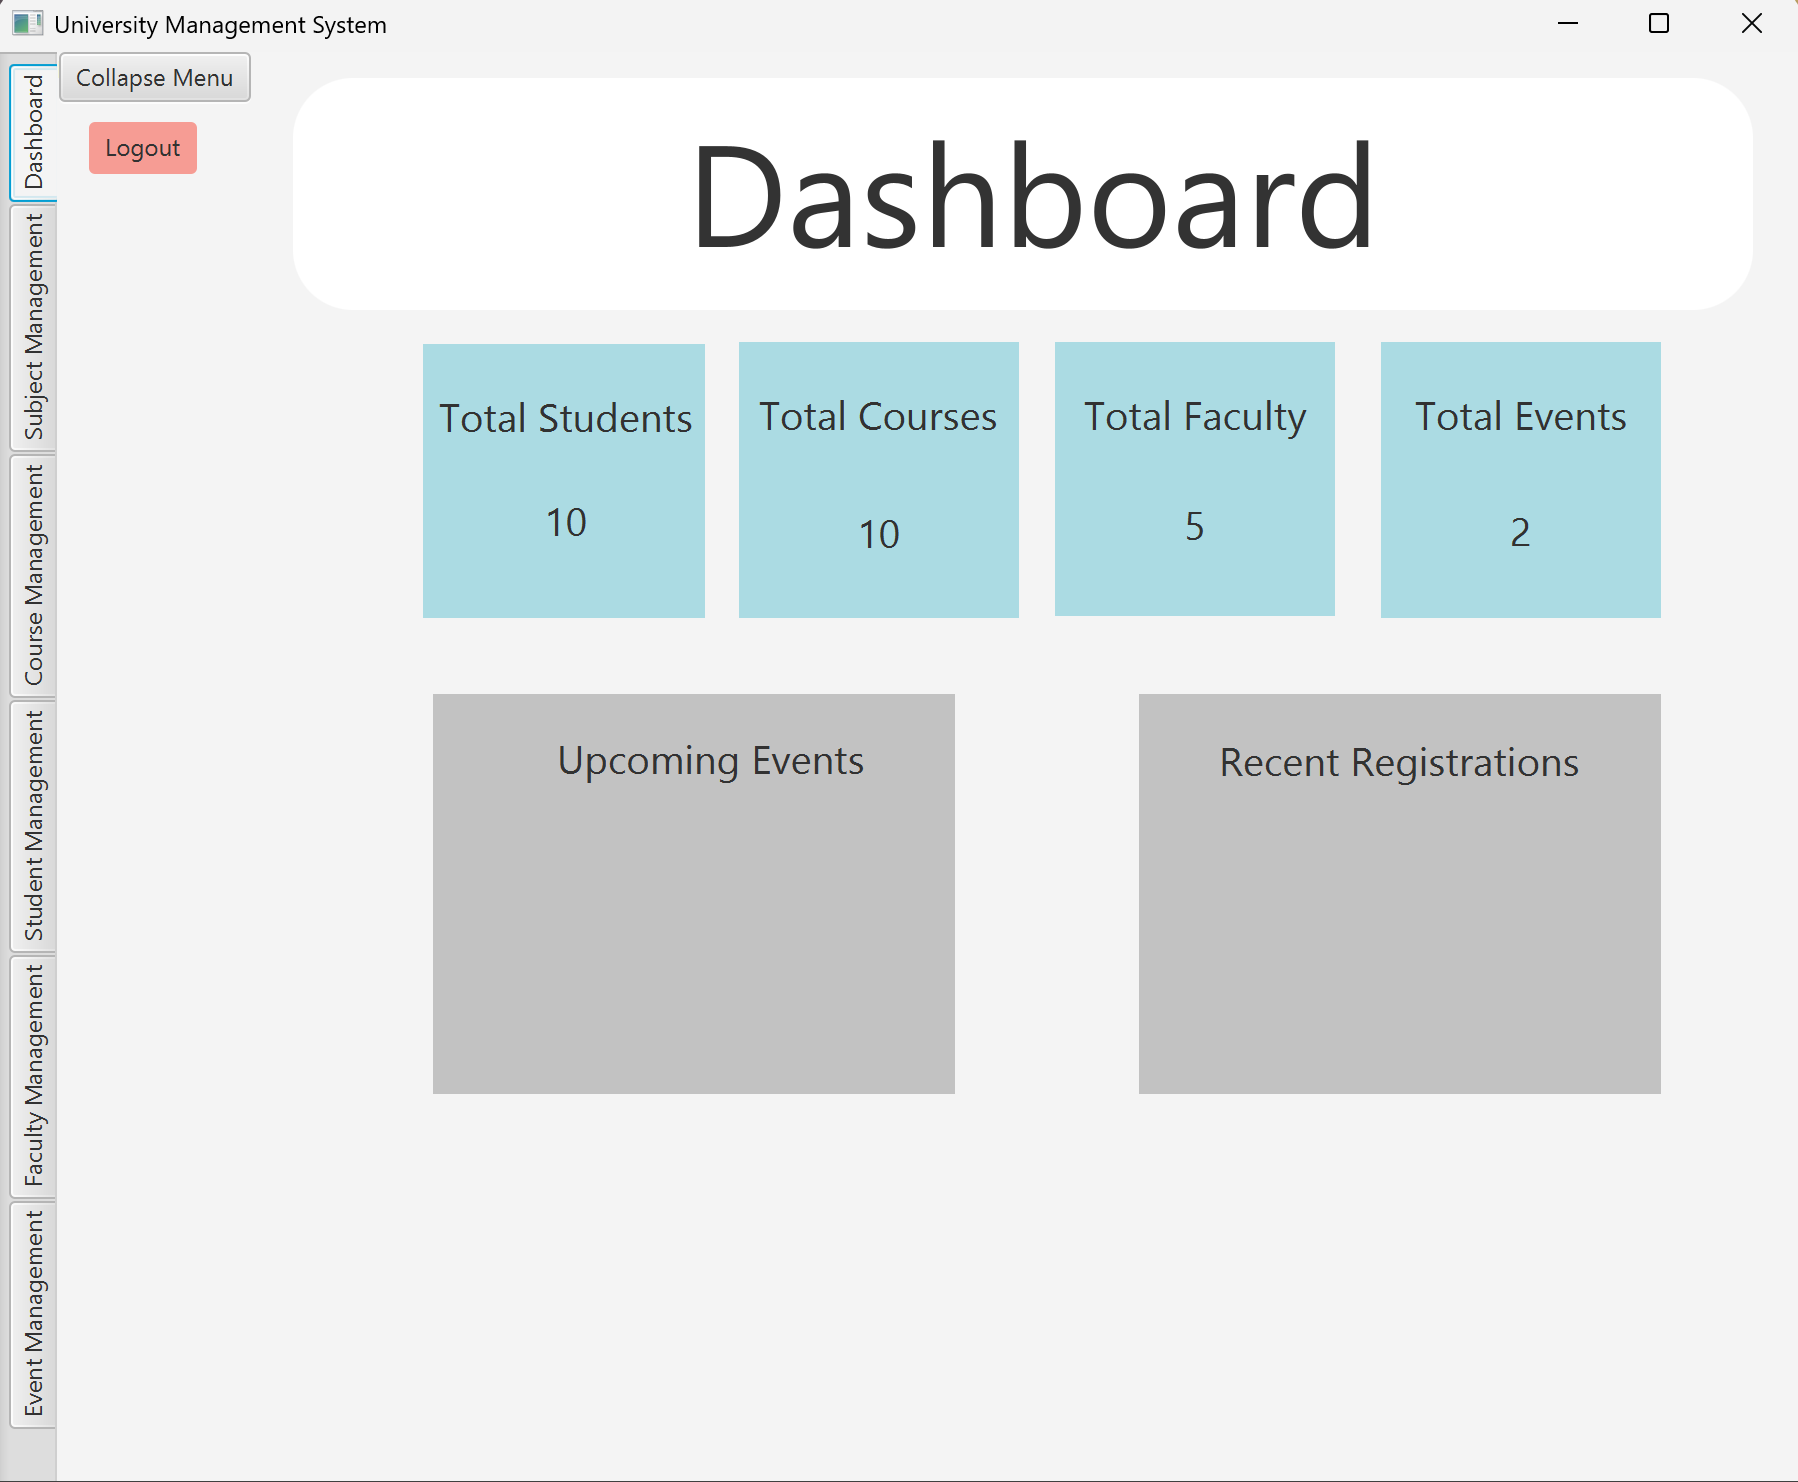
\includegraphics[width=1\linewidth]{figures/Dashboard.png}
%         \caption{Dashboard}
%         % \label{fig:example11}  
% \end{figure}


% \subsubsection{Faculty View}

% \begin{figure}[ht]
%     \centering
%         \centering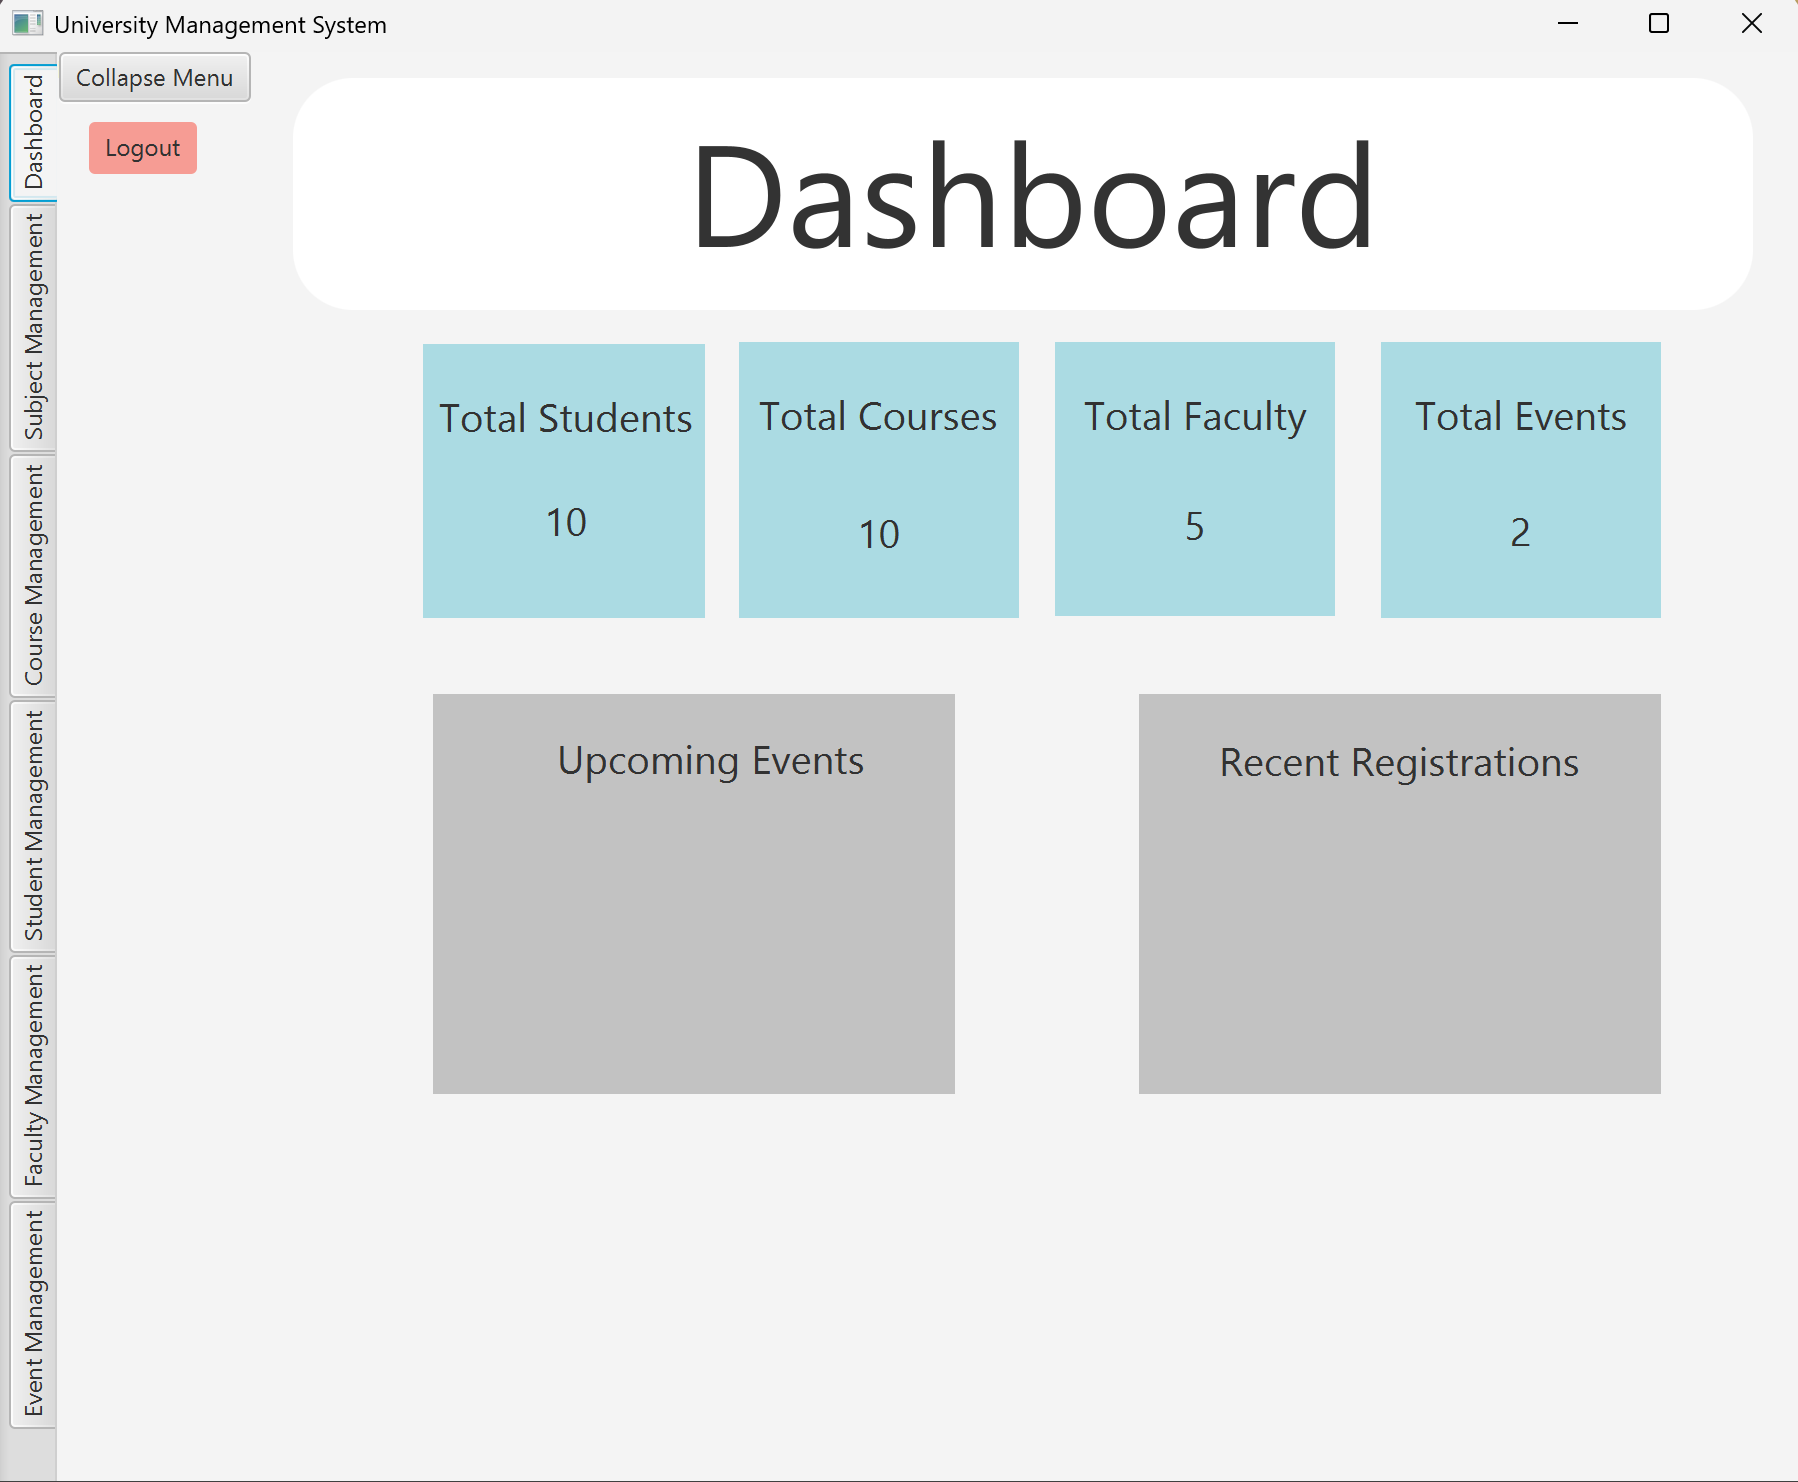
\includegraphics[width=1\linewidth]{figures/Dashboard.png}
%         \caption{Dashboard}
%         % \label{fig:example11}  
% \end{figure}


\newpage
\subsection{Faculty Management Tab}

\lipsum[9]

\subsubsection{Faculty View}

\lipsum[9]

\begin{figure}[ht!]
    \centering
        \centering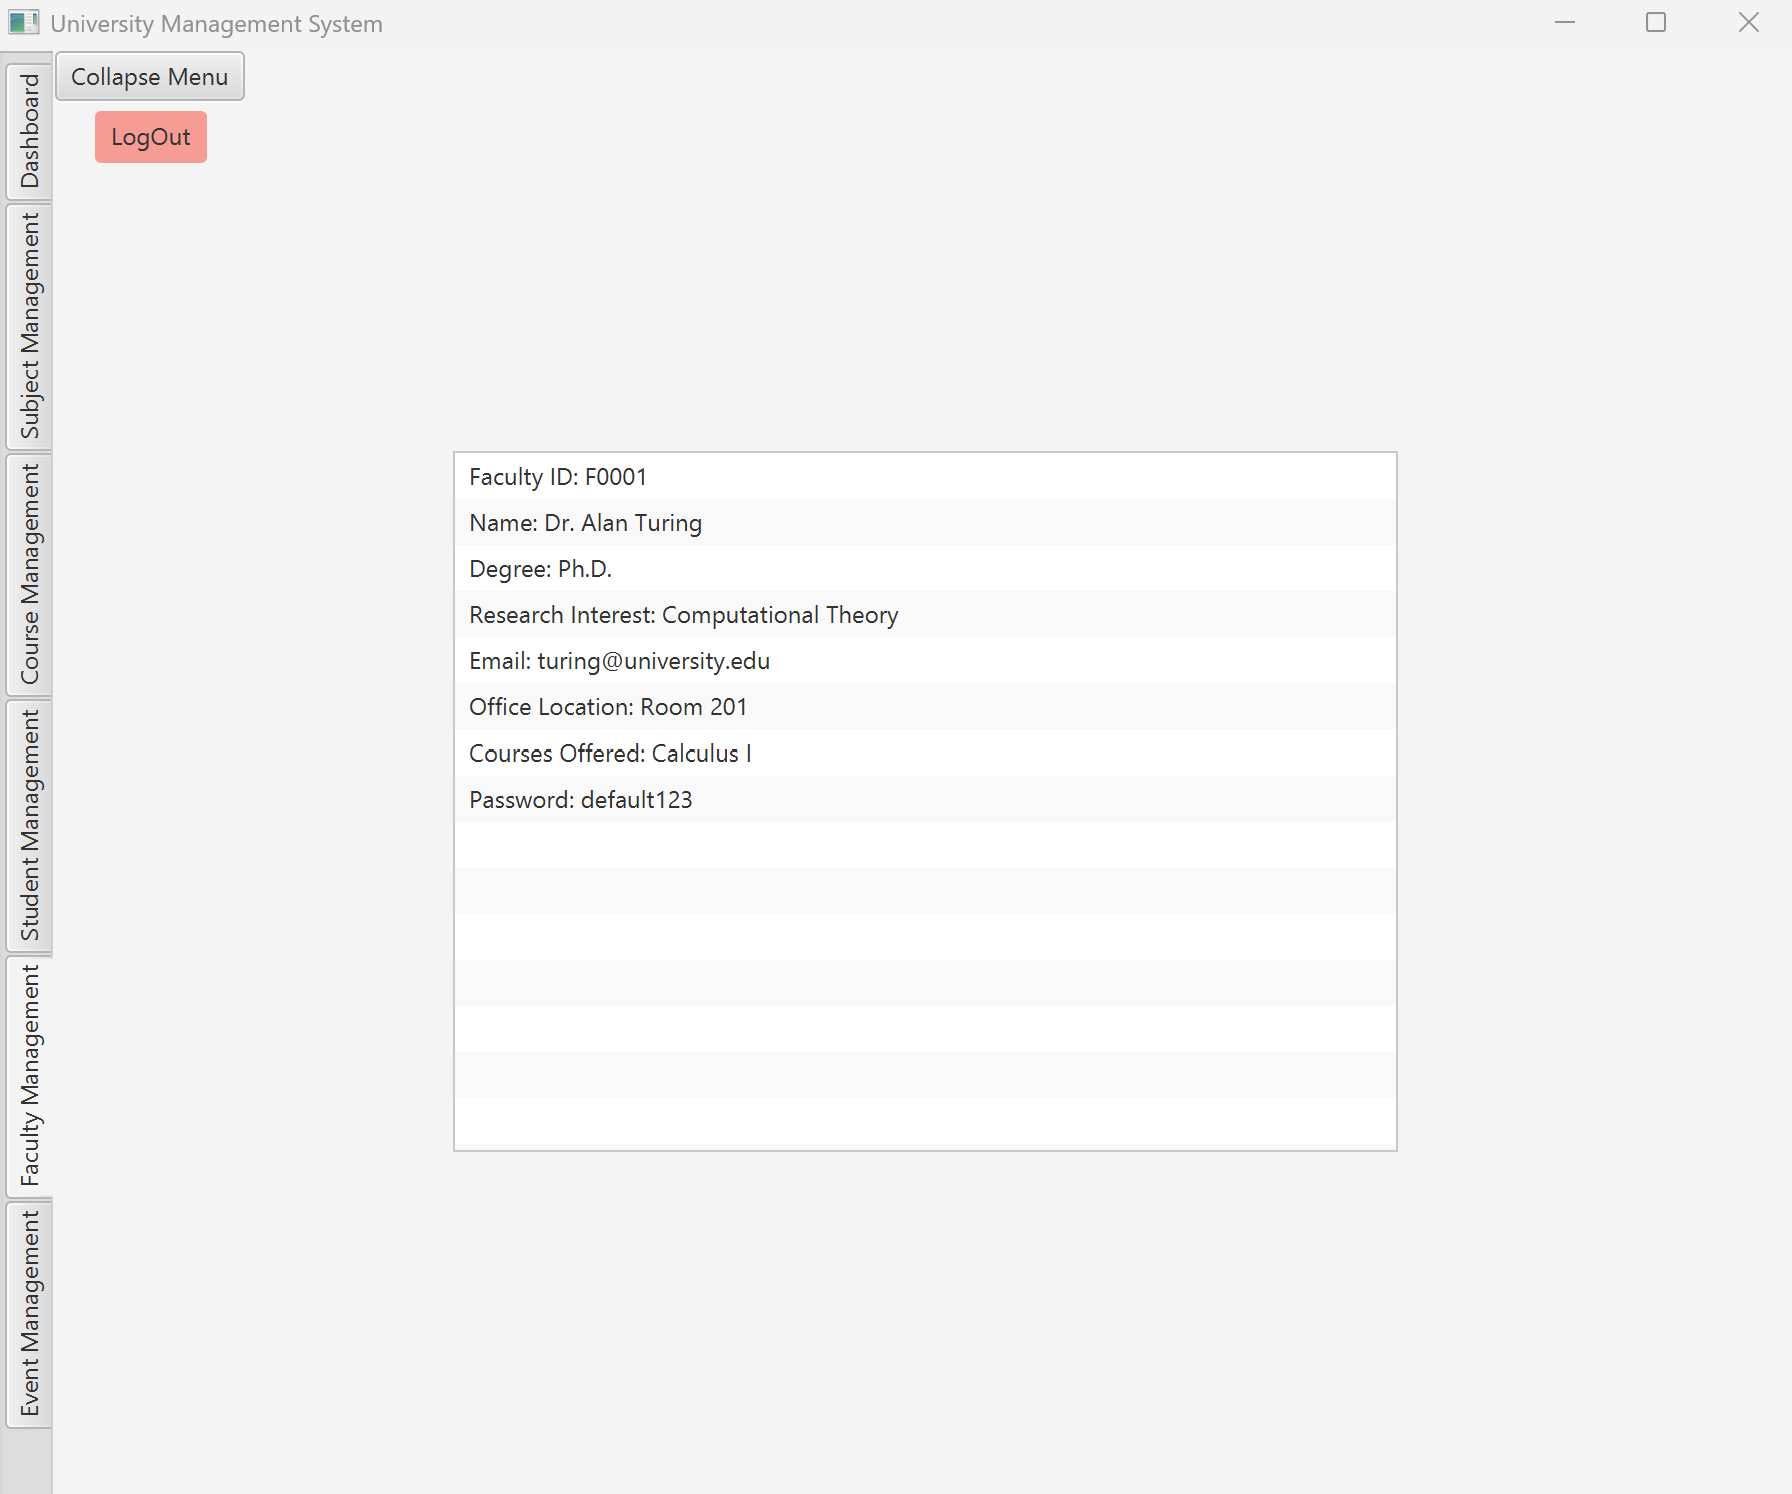
\includegraphics[width=0.7\linewidth]{figures/FAC_Faculty_Management_Tab.png}
        \caption{Faculty Login - Faculty Management}
        % \label{fig:example11}  
\end{figure}


\subsubsection{Student View}

\lipsum[9]

\begin{figure}[ht!]
    \centering
        \centering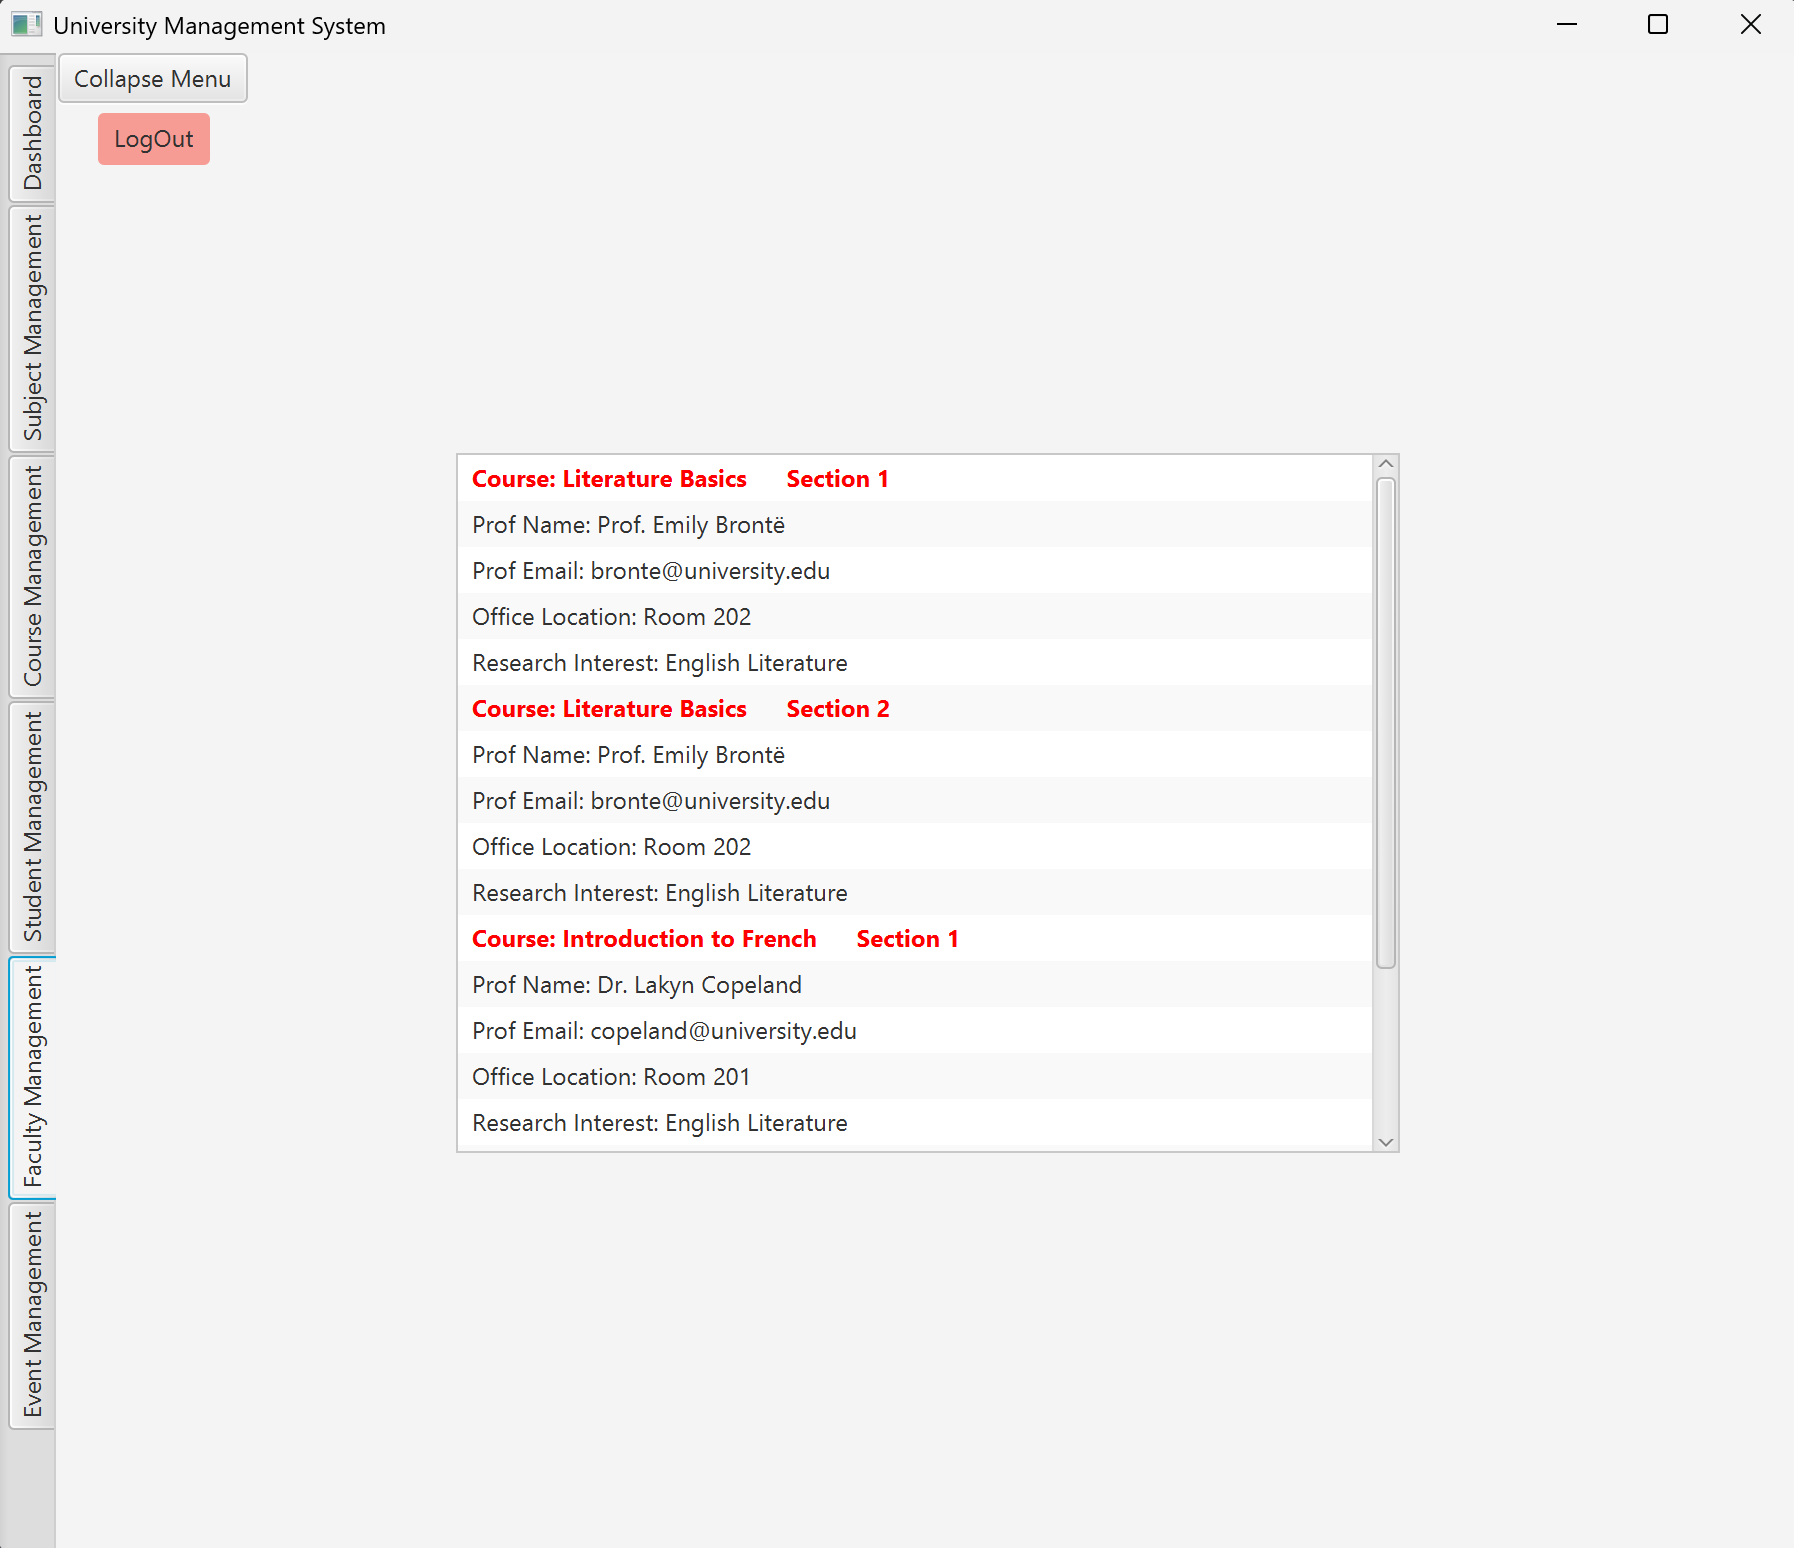
\includegraphics[width=0.8\linewidth]{figures/STD_Faculty_Tab.png}
2        \caption{Student Login - Faculty Management}
        % \label{fig:example11}  
\end{figure}



\newpage
\section{Troubleshooting \& Support}

Throughout the design of this program, there may be bugs that might have been an oversight. Troubleshooting continues to become a problem and in the test that was conducted for user experience, the main error issue that exists is logging into the UMS.  These bugs may require troubleshooting to fix the error (e.g., spelling or capitalization for logging in). Although the program aims to support and be bug-free, they might remain in the program and if they are persistent and affecting the experience. Contact the authors of the program for assistance.



\subsection{Common Login Issues}
Login issues can only arise when the user, faculty, student, or administrator, enters an incorrect username or password. If and when this occurs, a message will be prompted to inform the user that their inputted information is incorrect. It does not provide feedback on whether it is the password or the username.


\subsection{Frequently Asked Question}
\begin{enumerate}
    \item How many times can you attempt to login before it locks me out?
    \begin{itemize}
        \item The login menu will not lock out users if they continue to enter incorrect passwords and usernames.
    \end{itemize}
    \item Do faculty users have access to deleting students privileges
    \begin{itemize}
        \item Faculty users do not have the permission to delete student, only the administrators have access to complete this task.
    \end{itemize}
\end{enumerate}

% \subsection{Error Message \& Solutions (Optional)}
\newpage
\section{Class Library}  


\subsection*{Java Domain Classes (Source Listing)} 

\begin{comment}
    Place each class from the class library for verification purposes in the user guide
\end{comment}



\begin{lstlisting}[title={Admin Dashboard},language=Java,breaklines=true,postbreak=, breakatwhitespace=true, basicstyle=\ttfamily\small,columns=fullflexible]
package com.example.university_management;

import javafx.collections.FXCollections;
import javafx.collections.ObservableList;
import javafx.fxml.FXML;
import javafx.fxml.FXMLLoader;
import javafx.fxml.Initializable;
import javafx.scene.Parent;
import javafx.scene.Scene;
import javafx.scene.control.*;
import javafx.scene.control.cell.PropertyValueFactory;
import javafx.scene.input.KeyCode;
import javafx.scene.input.MouseEvent;
import javafx.scene.layout.FlowPane;
import javafx.scene.layout.StackPane;
import javafx.scene.layout.VBox;
import javafx.scene.paint.Color;
import javafx.scene.shape.Rectangle;
import javafx.scene.text.Text;
import javafx.stage.Stage;

import java.io.IOException;
import java.net.URL;
import java.time.*;
import java.time.format.DateTimeFormatter;
import java.util.*;
import java.util.concurrent.atomic.AtomicBoolean;

public class AdminDash implements Initializable {
    @FXML private TextField textEvent;
    @FXML private TableView<Course> courseInfo;
    @FXML private Button collapseButton;
    @FXML private Label totalEvents;
    @FXML private Label totalFaculty;
    @FXML private Label studentCountLabel;
    @FXML private Label totalCourses;
    @FXML
    private TableView<Student> studentTable;
    @FXML
    private TableColumn<Student, String> colmStudentID;
    @FXML
    private TableColumn<Student, String> colmStudentName;
    @FXML
    private TableColumn<Student, String> colmStudentEmail;
    @FXML private ListView<String> adminSubjects;
    @FXML private Button deleteSubjectBtn;
    @FXML private TabPane tabs;
    private static int counter = 0;
    ZonedDateTime today;
    ZonedDateTime dateFocus;
    @FXML private Text month; //links to text called month on dashboard.fxml
    @FXML private  Text year;
    @FXML private FlowPane calendar;
    @FXML private TableColumn<Course, String> courseCode; //all of these and bellow are different columns of the table
    @FXML private TableColumn<Course, String> courseName;
    @FXML private TableColumn<Course, String> subjectCode;
    @FXML private TableColumn<Course, String> sectionNumber;
    @FXML private TableColumn<Course, String> capacity;
    @FXML private TableColumn<Course, String> lectureTime;
    @FXML private TableColumn<Course, String> finalExam;
    @FXML private TableColumn<Course, String> location;
    @FXML private TableColumn<Course, String> teacherName;
    @FXML private ListView<String> facultyList;
    @FXML private Text studentText;
    @FXML private Button deleteCourses;
    @FXML private Label capacityLabel;
    @FXML private Slider capacitySlider;
    @FXML private Label costLabel;
    @FXML private Slider costSlider;
    @FXML private DatePicker addEventDate;
    @FXML private TextField eventName;
    @FXML private TextField eventLocation;
    @FXML private Button addEventBtn;
    @FXML private TextField eventNameField;
    @FXML private TextField eventLocationField;
    @FXML private Slider timeSlider;
    @FXML private  Label timeLabel;
    @FXML private ChoiceBox<String> coursesOffered;
    @FXML private ChoiceBox<String> degree;
    @FXML private Button addFaculty;
    @FXML private TextField facultyName;
    @FXML private TextField researchIntereset;
    @FXML private TextField officeLocation;
    static String name;
    static String address;
    static String telephone;
    static String email;
    private int counterText = 0;
    @FXML private Text eventText;
    @FXML
    public void initialize() {
        // Bind columns to Student properties
        colmStudentID.setCellValueFactory(new PropertyValueFactory<>("studentID"));
        colmStudentName.setCellValueFactory(new PropertyValueFactory<>("name"));
        colmStudentEmail.setCellValueFactory(new PropertyValueFactory<>("email"));

        // Load student data initially
        loadStudentData();

        // Handle double-click for opening student details
        studentTable.setOnMouseClicked(event -> {
            if (event.getClickCount() == 2) { // Double-click opens details
                Student selectedStudent = studentTable.getSelectionModel().getSelectedItem();
                if (selectedStudent != null) {
                    openStudentDetailsWindow(selectedStudent);
                }
            }
        });
        adminSubjects.setOnMouseClicked(mouseEvent ->  {
            String selectedItem = adminSubjects.getSelectionModel().getSelectedItem();
            if (selectedItem != null){
                deleteSubject(selectedItem);
            }
        });
    }

    private void openStudentDetailsWindow(Student student) {
        try {
            // Load FXML
            FXMLLoader loader = new FXMLLoader(getClass().getResource("StudentDetails.fxml"));
            Parent root = loader.load();

            // Get controller and pass student data
            StudentDetailsController controller = loader.getController();
            Stage detailsStage = new Stage();
            controller.setStudentDetails(student, detailsStage, this);

            // Setup stage
            detailsStage.setTitle("Student Details");
            detailsStage.setScene(new Scene(root));
            detailsStage.show();
        } catch (IOException e) {
            e.printStackTrace();
        }
    }

    private void loadStudentData() {
        ObservableList<Student> studentList = FXCollections.observableArrayList();

        // Get students from Excel or Reading_Student (already loaded from Excel)
        Student[] students = Reading_Student.getAllStudents();
        if (students != null) {
            studentList.addAll(students);
        }

        // Set the table's items to the observable list
        studentTable.setItems(studentList);
    }


    public void refreshTable(Student student) throws IOException {
        Reading_Student.loadStudentCredentials();
        loadStudentData();
        studentTable.getItems().remove(student);
        studentTable.refresh();
    }

    public void loadAdminSubject() throws IOException{
        adminSubjects.getItems().clear(); // Clear existing items
        ReadingSubject.loadSubjects(); // Load subjects from Excel
        Subject[] subjects = ReadingSubject.getAllSubjects(); // Retrieve subjects

        if (subjects == null || subjects.length == 0) {
            adminSubjects.getItems().add("No subjects available.");
            return;
        }

        for (Subject subj : subjects) {
            if (subj != null) {
                adminSubjects.getItems().add(subj.getCode() + " - " + subj.getName()); // Display formatted subject info
            }
        }
    }
    public void deleteSubject(String subjectDelete) {
        deleteSubjectBtn.setOnAction(actionEvent -> {
            try {
                deleteSubject.deletingSubject(subjectDelete.replaceAll("\\s.*", ""));
            } catch (IOException e) {
                throw new RuntimeException(e);
            }
            adminSubjects.getItems().remove(subjectDelete);

        });
    }
    public void collapseMenu(){
        if(counter ==0) {
            tabs.setVisible(false);
            counter+=1;
            collapseButton.setText("Open Menu");

        }
        else{
            tabs.setVisible(true);
            counter = 0;
            collapseButton.setText("Collapse Menu");
        }

    }
    public void initialize(URL url, ResourceBundle resourceBundle){
        dateFocus = ZonedDateTime.now(); //sets dateFocus to the current date
        today = ZonedDateTime.now();
        try { //creates calendar
            drawCalendar();
        } catch (IOException e) {
            throw new RuntimeException(e);
        }
        capacitySlider.valueProperty().addListener((observable, oldValue, newValue) -> {
            capacityLabel.setText("Capacity: " + Math.round(capacitySlider.getValue()));
        });
        costSlider.valueProperty().addListener((observable, oldValue, newValue) ->{
            costLabel.setText("Cost: " + String.format("%.2f", costSlider.getValue()));
        });
        timeSlider.valueProperty().addListener((observable, oldValue, newValue) -> {
            timeLabel.setText(String.format("%.2f", timeSlider.getValue()));
        });
        addEventBtn.setStyle("-fx-background-color: "
                + "linear-gradient(#f49794, #ff6666), "
                + "radial-gradient(center 50% -40%, radius 200%, #ff7f7f 45%, #b30000 50%); "
                + "-fx-background-radius: 6, 5; "
                + "-fx-background-insets: 0, 1; "
                + "-fx-effect: dropshadow(three-pass-box, rgba(0, 0, 0, 0.4), 5, 0.0, 0, 1); "
                + "-fx-text-fill: white; "
                + "-fx-font-weight: bold;");
    }
    @FXML
    void backOneMonth() throws IOException { //goes back one month
        dateFocus = dateFocus.minusMonths(1);
        calendar.getChildren().clear();
        drawCalendar();
    }
    @FXML
    void forwardOneMonth() throws IOException { //goes forward one month
        dateFocus = dateFocus.plusMonths(1);
        calendar.getChildren().clear();
        drawCalendar();
    }
    private void drawCalendar() throws IOException {
        year.setText(String.valueOf(dateFocus.getYear())); // Set year text
        month.setText(String.valueOf(dateFocus.getMonth())); // Set month text

        double calendarWidth = calendar.getPrefWidth();
        double calendarHeight = calendar.getPrefHeight();
        double strokeWidth = 2;
        double spacingH = calendar.getHgap();
        double spacingV = calendar.getVgap();

        Map<Integer, List<CalendarActivity>> calendarActivityMap = getCalendarActivitiesMonth(dateFocus);
        Map<Integer, StackPane> dateStackPaneMap = new HashMap<>(); // Store stack panes for each date

        int monthMaxDate = dateFocus.getMonth().maxLength();
        if (dateFocus.getYear() % 4 != 0 && monthMaxDate == 29) {
            monthMaxDate = 28;
        }
        int dateOffset = ZonedDateTime.of(dateFocus.getYear(), dateFocus.getMonthValue(), 1, 0, 0, 0, 0, dateFocus.getZone()).getDayOfWeek().getValue();

        for (int i = 0; i < 6; i++) {
            for (int j = 0; j < 7; j++) {
                StackPane stackPane = new StackPane();
                Rectangle rectangle = new Rectangle();
                rectangle.setArcWidth(30);
                rectangle.setArcHeight(30);
                rectangle.setFill(Color.rgb(255, 99, 71, 0.5));
                rectangle.setStroke(Color.BLACK);
                rectangle.setOnMouseEntered(event -> rectangle.setFill(Color.LIGHTBLUE));
                rectangle.setOnMouseExited(event -> rectangle.setFill(Color.rgb(255, 99, 71, 0.5)));
                rectangle.setStrokeWidth(strokeWidth);
                double rectangleWidth = (calendarWidth / 7) - strokeWidth - spacingH;
                rectangle.setWidth(rectangleWidth);
                double rectangleHeight = (calendarHeight / 6) - strokeWidth - spacingV;
                rectangle.setHeight(rectangleHeight);
                stackPane.getChildren().add(rectangle);

                int calculatedDate = (j + 1) + (7 * i);

                rectangle.setOnMousePressed(event -> {
                    if (calculatedDate - dateOffset > 0 && calculatedDate - dateOffset <= dateFocus.getMonth().maxLength()) {
                        LocalDate selectedDate = LocalDate.of(dateFocus.getYear(), dateFocus.getMonthValue(), calculatedDate - dateOffset);
                        addEventDate.setValue(selectedDate);
                    }
                });

                if (calculatedDate > dateOffset) {
                    int currentDate = calculatedDate - dateOffset;
                    if (currentDate <= monthMaxDate) {
                        Text date = new Text(String.valueOf(currentDate));
                        double textTranslationY = -(rectangleHeight / 2) * 0.75;
                        date.setFill(Color.rgb(59, 69, 1, 0.95));
                        date.setTranslateY(textTranslationY);
                        stackPane.getChildren().add(date);

                        dateStackPaneMap.put(currentDate, stackPane); // Store stackPane for this date

                        List<CalendarActivity> calendarActivities = calendarActivityMap.get(currentDate);
                        if (calendarActivities != null) {
                            createCalendarActivity(calendarActivities, rectangleHeight, rectangleWidth, stackPane);
                        }
                    }
                    if (today.getYear() == dateFocus.getYear() && today.getMonth() == dateFocus.getMonth() && today.getDayOfMonth() == currentDate) {
                        rectangle.setStroke(Color.BLUE);
                    }
                }
                calendar.getChildren().add(stackPane);
            }
        }

        addEventBtn.setOnAction(event -> {
            LocalDate selectedDate = addEventDate.getValue();
            String eventName = eventNameField.getText();
            String eventLocation = eventLocationField.getText();
            String time = timeLabel.getText();
            String eventCapacity = String.valueOf(Math.round(capacitySlider.getValue()));
            String eventCost = String.valueOf(costSlider.getValue());
            DateTimeFormatter timeFormatter = DateTimeFormatter.ofPattern("HH:mm");
            String formattedTime = time.replace(".", ":");
            LocalTime localTime = LocalTime.parse(formattedTime, timeFormatter);

            if (selectedDate != null && eventName != null && !eventName.isEmpty() && !eventLocation.isEmpty()) {
                ZonedDateTime eventDateTime = ZonedDateTime.of(selectedDate, localTime, ZoneId.systemDefault());
                eventNameField.clear();
                eventLocationField.clear();
                addEventDate.setValue(null);
                DateTimeFormatter formatter = DateTimeFormatter.ofPattern("MM/dd/yyyy HH:mm");
                String formatedDate = eventDateTime.format(formatter);
                Event.addEvent(eventName, "No Description",eventLocation, String.valueOf(formatedDate),eventCapacity, eventCost );
                StackPane selectedStackPane = dateStackPaneMap.get(selectedDate.getDayOfMonth());
                if (selectedStackPane != null) {
                    CalendarActivity activity = new CalendarActivity(eventDateTime, eventName, eventLocation);
                    List<CalendarActivity> calendarActivities = calendarActivityMap.computeIfAbsent(selectedDate.getDayOfMonth(), k -> new ArrayList<>());
                    calendarActivities.add(activity);

                    // Remove duplicate event title and use only createCalendarActivity
                    selectedStackPane.getChildren().removeIf(node -> node instanceof VBox);
                    createCalendarActivity(calendarActivities, (calendarHeight / 6) - strokeWidth - spacingV, (calendarWidth / 7) - strokeWidth - spacingH, selectedStackPane);
                }
            }
        });
    }
    private void createCalendarActivity(List<CalendarActivity> calendarActivities, double rectangleHeight, double rectangleWidth, StackPane stackPane) {
        VBox calendarActivityBox = new VBox();
        calendarActivityBox.setSpacing(2);
        calendarActivityBox.setMaxWidth(rectangleWidth * 0.9);
        calendarActivityBox.setMaxHeight(rectangleHeight * 0.8);
        for (int k = 0; k < calendarActivities.size(); k++) {
            if (k >= 2) {
                Text moreActivities = new Text("...");
                calendarActivityBox.getChildren().add(moreActivities);
                break;
            }
            Text text = new Text(calendarActivities.get(k).getClientName() + ", " + calendarActivities.get(k).getDate().toLocalTime());
            text.setWrappingWidth(rectangleWidth * 0.85); // Prevent text overflow
            text.setStyle("-fx-font-size: 12px; -fx-fill: black;"); // Make text visible

            int finalK = k;
            text.setOnMouseClicked(mouseEvent -> {
                System.out.println(text.getText());
                try {
                    FXMLLoader loader = new FXMLLoader(getClass().getResource("eventDetails.fxml"));
                    Parent root = loader.load();
                    EventDetailsController controller = loader.getController();
                    Stage detailsStage = new Stage();
                    controller.setEventDetails(calendarActivities.get(finalK).getClientName(), this);

                    detailsStage.setTitle("Event Details");
                    detailsStage.setScene(new Scene(root));
                    detailsStage.show();
                } catch (IOException e) {
                    e.printStackTrace();
                }
            });
            text.setOnMouseEntered(mouseEvent -> text.setStyle("-fx-font-size: 12px; -fx-fill: #ae4802;"));
            text.setOnMouseExited(mouseEvent -> text.setStyle("-fx-font-size: 12px; -fx-fill: black;"));
            calendarActivityBox.getChildren().add(text);
        }
        calendarActivityBox.setTranslateY((rectangleHeight / 2) * 0.20);
        stackPane.getChildren().add(calendarActivityBox);
    }

    private Map<Integer, List<CalendarActivity>> createCalendarMap(List<CalendarActivity> calendarActivities) {
        Map<Integer, List<CalendarActivity>> calendarActivityMap = new HashMap<>();

        for (CalendarActivity activity: calendarActivities) {
            int activityDate = activity.getDate().getDayOfMonth();
            if(!calendarActivityMap.containsKey(activityDate)){
                calendarActivityMap.put(activityDate, List.of(activity));
            } else {
                List<CalendarActivity> OldListByDate = calendarActivityMap.get(activityDate);

                List<CalendarActivity> newList = new ArrayList<>(OldListByDate);
                newList.add(activity);
                calendarActivityMap.put(activityDate, newList);
            }
        }
        return  calendarActivityMap;
    }

    private Map<Integer, List<CalendarActivity>> getCalendarActivitiesMonth(ZonedDateTime dateFocus) throws IOException {
        List<CalendarActivity> calendarActivities = new ArrayList<>();
        ReadEvents.loadEvents();
        Event[] event = ReadEvents.getAllEvents();
        for (Event event1 : event) {
            // Ensure event1 is not null and its dateAndTime is valid
            if (event1 == null || event1.dateAndTime == null || event1.dateAndTime.trim().isEmpty()) {
                continue;  // Skip if invalid
            }

            // Parse the event's dateAndTime into LocalDateTime first
            DateTimeFormatter formatter = DateTimeFormatter.ofPattern("MM/dd/yyyy HH:mm");
            LocalDateTime localDateTime = LocalDateTime.parse(event1.dateAndTime, formatter);

            // Convert LocalDateTime to ZonedDateTime by adding a time zone
            ZonedDateTime eventDateTime = localDateTime.atZone(ZoneId.systemDefault()); // Adjust time zone as needed

            // Extract the month and year from the event's date and the dateFocus
            int eventMonth = eventDateTime.getMonthValue();  // Get the event's month (1-12)
            int eventYear = eventDateTime.getYear();         // Get the event's year

            int focusMonth = dateFocus.getMonthValue();     // Get the focus month's value
            int focusYear = dateFocus.getYear();            // Get the focus year

            // Check if the event's month and year match the month and year of dateFocus
            if (eventMonth == focusMonth && eventYear == focusYear) {
                // If the event is in the same month as dateFocus, add it to the calendar
                ZonedDateTime time = getDateTime(dateFocus, event1, formatter);
                calendarActivities.add(new CalendarActivity(time, event1.eventName, event1.location));
            }
        }
        return createCalendarMap(calendarActivities);
    }

    private static ZonedDateTime getDateTime(ZonedDateTime dateFocus, Event event1, DateTimeFormatter formatter) {
        LocalDateTime dateTime = LocalDateTime.parse(event1.dateAndTime.trim(), formatter);
        int day = dateTime.getDayOfMonth();
        int year = dateTime.getYear();
        int month = dateTime.getMonthValue();
        int hour = dateTime.getHour();
        int minute = dateTime.getMinute();
        int second = dateTime.getSecond();
        ZoneId zone = dateFocus.getZone();
        return ZonedDateTime.of(year, month,day, hour, minute, second,0,zone);
    }
    @FXML
    private void loadCourseInfo() throws IOException {
        ReadingCourses.loadCourses();
        courseCode.setCellValueFactory(new PropertyValueFactory<>("courseCode"));
        courseName.setCellValueFactory(new PropertyValueFactory<>("courseName"));
        subjectCode.setCellValueFactory(new PropertyValueFactory<>("subjectCode"));
        sectionNumber.setCellValueFactory(new PropertyValueFactory<>("sectionNumber"));
        capacity.setCellValueFactory(new PropertyValueFactory<>("capacity"));
        lectureTime.setCellValueFactory(new PropertyValueFactory<>("lectureTime"));
        finalExam.setCellValueFactory(new PropertyValueFactory<>("finalExamDate"));
        location.setCellValueFactory(new PropertyValueFactory<>("location"));
        teacherName.setCellValueFactory(new PropertyValueFactory<>("teacherName"));
        ObservableList<Course> courseList = FXCollections.observableArrayList();
        Course[] courses = ReadingCourses.getAllCourseInfo();
        for(Course course1: courses){
            if(!(course1.courseName.isEmpty())){
                courseList.add(course1);
            }
        }
        String code;
        final Course[] selectedCourse = new Course[1];
        courseInfo.setItems(courseList);
        courseInfo.setOnMouseClicked(event -> {
            if (event.getClickCount() == 2) { // Double-click opens details
                selectedCourse[0] = courseInfo.getSelectionModel().getSelectedItem();
                deleteCourses.setText("Delete "+ selectedCourse[0].courseName);

            }
        });
        deleteCourses.setOnAction(event -> {

            try {
                Course.deleteCourse(selectedCourse[0].courseName);
            } catch (IOException e) {
                throw new RuntimeException(e);
            }
            courseInfo.getItems().remove(selectedCourse[0]);
            deleteCourses.setText("Delete Subject");
        });
    }
    @FXML
    public void faculty() throws IOException {
        facultyList.getItems().clear();
        ReadingFaculties.loadFaculties();
        Faculties[] faculties = ReadingFaculties.getAllFaculty();
        for (Faculties faculties1 : faculties) {
            if (faculties1 == null) {
                continue;
            }
            if (!(faculties1.name.isEmpty())) {
                facultyList.getItems().add("Name: " + faculties1.name + "         ID: " + faculties1.ID);
            }
        }
        facultyList.setOnMouseClicked(event -> {
            String selectedItem = facultyList.getSelectionModel().getSelectedItem();
            try {
                ReadingFaculties.loadFaculties();
            } catch (IOException e) {
                throw new RuntimeException(e);
            }
            try {
                FXMLLoader loader = new FXMLLoader(getClass().getResource("facultyDetails.fxml"));
                Parent root = loader.load();

                // Get controller and pass student data
                String name = selectedItem.replaceFirst(".*ID:", "").trim();
                facultyDetailsController controller = loader.getController();
                Stage detailsStage = new Stage();
                System.out.println(name);
                controller.setFacultyDetails(name, this);

                detailsStage.setTitle("Faculty Details");
                detailsStage.setScene(new Scene(root));
                detailsStage.show();
            } catch (IOException e) {
                e.printStackTrace();
            }
        });
        coursesOffered.getItems().clear();
        coursesOffered.setValue("Select Course Offered");
        coursesOffered.getItems().add("Select Courses Offered");
        ReadingCourses.loadCourses();
        Course[] courses = ReadingCourses.getAllCourseInfo();
        Set<String> seenNames = new HashSet<>();
        degree.getItems().clear();
        degree.setValue("Select Degree");
        degree.getItems().add("Select Degree");
        degree.getItems().add("Ph.D");
        degree.getItems().add("Master's");
        for (Course course : courses) {
            if (seenNames.add(course.courseName)) {
                // If courseName is new, add to coursesOffered
                coursesOffered.getItems().add(course.courseName);
            }
        }

        coursesOffered.getItems().removeLast();
        addFaculty.setOnAction(MouseEvent ->{
            String newId = null;
            for (Faculties faculties1 : faculties) {
                if (faculties1 == null){
                    break;
                }
                int number = Integer.parseInt(faculties1.ID.substring(1));
                number++;
                newId = String.format("F%04d", number);
            }
            int lastSpace = facultyName.getText().lastIndexOf(" ");
            String lastName = facultyName.getText().substring(lastSpace+1);

            Faculties faculty = new Faculties(newId, facultyName.getText(), degree.getValue(), researchIntereset.getText(), lastName.toLowerCase() + "@university.edu", officeLocation.getText(), coursesOffered.getValue(), "default123");
            facultyList.getItems().add("Name: " + faculty.name + "         ID: " + faculty.ID);
            Faculties.addFaculty(faculty);
        });
    }
    @FXML
    private void countingStudents() throws IOException {
        Reading_Student.loadStudentCredentials();
        Student[] list = Reading_Student.getAllStudents();
        int count1 =0;
        for (Student student1: list){
            if (!(student1.name.isEmpty())){
                count1+=1;
            }
        }
        studentCountLabel.setText(String.valueOf(count1));
        ReadingCourses.loadCourses();
        Course[] list1 = ReadingCourses.getAllCourseInfo();
        int count2 = 0;
        for(Course course: list1){
            if(!(course.courseName.isEmpty())){
                count2+=1;
            }
        }
        totalCourses.setText(String.valueOf(count2));
        ReadingFaculties.loadFaculties();
        Faculties[] list2 = ReadingFaculties.getAllFaculty();
        int count3 = 0;
        for (Faculties faculties: list2){
            if (faculties == null)continue;
            if(!(faculties.ID.isEmpty())) count3+=1;
        }
        totalFaculty.setText(String.valueOf(count3));
        ReadEvents.loadEvents();
        Event[] list3 = ReadEvents.getAllEvents();
        int count4 = 0;
        for(Event event: list3){
            if (event == null) continue;
            if(!(event.eventName.isEmpty())) count4 +=1;
        }
        totalEvents.setText(String.valueOf(count4));
    }
    private void addEvent(){
        String academicLevel = "Undergraduate";
        String currSem = "Fall 2025";
        String profilePhoto = "default";
        String subjRej = "";
        String thesis = "";
        String progress = "0%";
        AddStudent student = new AddStudent("", "default123", name, address, telephone, email, academicLevel, currSem, profilePhoto, subjRej, thesis, progress);
        student.addStudent();
        int index = studentTable.getItems().size() -1;
        studentTable.getItems().add(index,student);
        studentTable.refresh();

    }
    @FXML
    private void clearText(){
        textEvent.setOnKeyPressed(keyEvent -> {
            if (!textEvent.getText().isEmpty()){
                if(keyEvent.getCode() == KeyCode.ENTER) {
                    fields();
                    textEvent.clear();
                    counterText++;
                }
            }
                });
    }
    private void fields() {
        switch (counterText) {
            case 0:
                name = textEvent.getText();
                eventText.setText("Enter Address");
                studentText.setText("Name: " + name);
                break;
            case 1:
                address = textEvent.getText();
                eventText.setText("Enter Telephone");
                studentText.setText("Name: " + name +"  Address: " + address);
                break;
            case 2:
                telephone = textEvent.getText();
                eventText.setText("Enter Email");
                studentText.setText("Name: " + name +"  Address: " + address +"     Telephone: " + telephone);
                break;
            case 3:
                email = textEvent.getText();
                eventText.setText("Enter Name");
                studentText.setText("");
                addEvent();
                break;
        }
    }
    @FXML
    private void logOut() throws IOException {
        Stage stage = (Stage) deleteSubjectBtn.getScene().getWindow();
        stage.close();
        FXMLLoader fxmlLoader = new FXMLLoader(loginScreen.class.getResource("login.fxml")); //references the fxml called login
        Scene scene = new Scene(fxmlLoader.load(), 700, 500); //open login.fxml with dimensions 700 width and 500 height
        stage.setTitle("University Management System"); //sets the login screen title to university management system
        stage.setScene(scene);
        stage.show();

    }
    public void refreshEvents() throws IOException {
        calendar.getChildren().clear();
        drawCalendar();
    }
}
\end{lstlisting}



% \begin{lstlisting}[title={Admin Dashboard},language=Java,breaklines=true,postbreak=, breakatwhitespace=true, basicstyle=\ttfamily\small,columns=fullflexible]


% \end{lstlisting}












% \begin{figure}[ht]
%     \centering
%         \centering
\includegraphics[width=1\linewidth]{placeholder}
%         \caption{An example of multiple figures in one frame.}
%         \label{fig:example11}  
% \end{figure}



% \section{Results (optional)}

% \begin{figure}[ht]
%     \centering
%     \begin{subfigure}[t]{0.4\textwidth}
%         \centering
\includegraphics[width=1\linewidth]{placeholder}
%         \caption{An example of multiple figures in one frame.}
%         \label{fig:example11}
%     \end{subfigure}
%     %
%     \begin{subfigure}[t]{0.4\textwidth}
%         \centering
\includegraphics[width=1\linewidth]{placeholder}
%         \caption{Next subfigure.}
%         \label{fig:example12}
%     \end{subfigure}
%     %
%     \\
%     \begin{subfigure}[t]{0.4\textwidth}
%         \centering
\includegraphics[width=1\linewidth]{placeholder}
%         \caption{Subfigure on another line.}
%         \label{fig:example21}
%     \end{subfigure}
%     %
%     \begin{subfigure}[t]{0.4\textwidth}
%         \centering
\includegraphics[width=1\linewidth]{placeholder}
%         \caption{Yet another subfigure.}
%         \label{fig:example22}
%     \end{subfigure}    
% \end{figure}

% \lipsum[9]





%----------------------------------------------------------------------------------------
%	Bibliography
% %----------------------------------------------------------------------------------------
% \bibliography{bibliography/sample}{}
% \bibliographystyle{plain}

\end{document}